%% ==============================
\chapter{\iflanguage{ngerman}{Konzept}{Concept}}
\label{cha:konzept}
%% ==============================

Das Ziel dieses Kapitels ist es, eine HCS-basierte Alternative zur Ledger-Schicht der Referenzarchitektur von Erler et al.~\cite{erler2023} zu konzipieren, die deren Funktionen erfüllt, ohne die darüber liegende Agenten- und Kommunikationsschicht zu ändern. Damit wird die im Kapitel~\ref{cha:state_of_the_art} identifizierte Forschungslücke in einen konkreten Entwurf überführt, dessen Implementierung und Evaluation der Gegenstand der folgenden Kapitel sind.

Das Kapitel gliedert sich wie folgt: der Abschnitt~\ref{sec:konzipierung-referenzarchitektur} analysiert die Ausgangssituation, indem der Schnitt zwischen Agenten- und Ledger-Schicht klar definiert, die Funktionen der Ledger-Schicht systematisch identifiziert und ihren Hyperledger-Indy-spezifischen Mechanismen zugeordnet sowie der Umfang des geplanten Austauschs abgegrenzt wird. Der Abschnitt~\ref{sec:konzipierung-anforderungen} leitet daraus die funktionalen Anforderungen sowie die nicht-funktionalen Anforderungen ab. Der Abschnitt~\ref{sec:konzipierung-entwurf} trifft auf dieser Grundlage die Entwurfsentscheidungen für die HCS-basierte Ledger-Schicht. Der Abschnitt~\ref{sec:konzipierung-zielarchitektur} führt diese Entscheidungen zur Zielarchitektur zusammen, der Abschnitt~\ref{sec:konzipierung-evaluationskonzept} legt das Evaluationskonzept fest, und der Abschnitt~\ref{sec:konzipierung-zusammenfassung} fasst die Ergebnisse des Kapitels zusammen.

\section{Ausgangssituation und Analyse der Referenzarchitektur}
\label{sec:konzipierung-referenzarchitektur}

Der Ausgangspunkt der Konzipierung ist die im Abschnitt~\ref{sec:sota_referenzarchitektur} vorgestellte Referenzarchitektur für dezentrales Gesundheitsdatenmanagement nach Erler et al.~\cite{erler2023}. Das Ziel dieses Abschnitts besteht nicht darin, die Gesamtarchitektur erneut zu beschreiben, sondern eine gezielte Analyse der Architekturschicht, die im Rahmen dieser Arbeit ersetzt wird: der Ledger-Schicht. Dazu wird zuerst der für diese Analyse relevante Schnitt zwischen Agenten- und Ledger-Schicht gezogen und die Schnittstelle zwischen beiden bestimmt, anschließend werden die Funktionen der Ledger-Schicht systematisch identifiziert und den zugrunde liegenden Mechanismen von Hyperledger Indy zugeordnet. Abschließend wird der Umfang des geplanten Austauschs bestimmt.
Zur späteren Analyse wird zwischen den Funktionen unterschieden, die die Referenzarchitektur der Ledger-Schicht zuweist~\cite{erler2023}, und den Indy-spezifischen Mechanismen, mit denen diese Funktionen implementiert werden; letztere werden auf der Grundlage von Torongo und Toorani~\cite{torongo2023} beschrieben, da Erler et al. die internen Ledger-Komponenten nicht im Detail berücksichtigen.

Die Referenzarchitektur kann anhand der Taxonomie von Erler et al. ~\cite{erler2024} genau charakterisiert werden, in der die Autorinnen und Autoren ihren eigenen Entwurf einordnen \cite{erler2024}. Die Gesundheitsdaten bleiben off-chain und dezentral in den internen Systemen der datenhaltenden medizinischen Einrichtungen; als Ledger dient eine public permissioned Blockchain \cite{erler2023}. Das Identitätsmanagement folgt dem SSI-Paradigma mit nutzerzentrierter Komponente, da das Credential Wallet lokal durch ein Passwort abgesichert wird. Die Zugriffskontrolle liegt vollständig beim Patienten und wird über eine feingranulare DAC-Logik umgesetzt; die Zugriffsgewährung erfolgt über Tokenization in Kombination mit digitalen Signaturen innerhalb der DIDComm-Kommunikation \cite{erler2024}. Diese Einordnung benennt Eigenschaften, die eine HCS-basierte Alternative der Ledger-Schicht erhalten muss: Der Ledger funktioniert in der Referenzarchitektur ausschließlich als Vertrauensanker und Identitätsverzeichnis, nicht als Speicherort für Gesundheitsdaten.

\subsection{Schichtenschnitt und Schnittstelle zwischen den Schichten}
\label{subsec:schichtenstruktur}
Für die Analyse wird die im Abschnitt~\ref{sec:sota_referenzarchitektur} beschriebene Architektur in zwei Schichten unterteilt. Entscheidend für diesen Schnitt ist die Frage, welche Komponenten von einem Austausch der Ledger-Technologie überhaupt betroffen werden. Die Agenten-Schicht umfasst die DIDComm-basierte Peer-to-Peer-Kommunikation zwischen den Aries-Agenten der Patientenanwendung und der Netzwerk-Konnektoren einschließlich der Mediator-Infrastruktur; sie basiert auf paarweisen Peer-DIDs, die nicht auf dem Ledger registriert werden. Die Ledger-Schicht ergänzt diese Kommunikation um einen öffentlichen Vertrauensanker, der in der Referenzarchitektur durch eine public permissioned Hyperledger-Indy-Blockchain implementiert ist. ~\cite{erler2023}

Für diese Arbeit ist die Zusammensetzung der beiden Schichten nicht so wichtig, sondern die Schnittstelle zwischen ihnen, denn sie bestimmt, welche Operationen eine alternative Ledger-Implementierung bereitstellen muss. Aus der Aufgabenzuweisung der Referenzarchitektur~\cite{erler2023} ergeben sich drei Berührungspunkte, die sich direkt aus dem Lebenszyklus eines Credentials ablesen lassen (Abschnitt~\ref{sec:grundlagen-beispiel}, zusammengefasst in Tabelle~\ref{tab:beispiel-ledgerzugriffe}): das Veröffentlichen der öffentlichen Identitätsobjekte in der Vorbereitungsphase, das Auflösen dieser Objekte bei der Ausstellung und Präsentation und das Veröffentlichen des Widerrufsstatus. Der erste und der dritte Berührungspunkt sind schreibend, der zweite lesend; die Verbindungsphase kommt ohne Ledger-Zugriff aus, da Peer-DIDs nicht öffentlich registriert werden. Das Verhältnis von zwei lesenden zu einem schreibenden Zugriffszeitpunkt begründet, warum der Leseweg im weiteren Verlauf des Kapitels die zentrale Rolle einnimmt. Die Abbildung~\ref{fig:schichtenschnitt} stellt diesen Schnitt mit seinen drei Berührungspunkten dar. Diese drei Berührungspunkte bilden den operativen Kern der Schnittstelle, die eine alternative Ledger-Implementierung bereitstellen muss. Sie werden im folgenden Abschnitt um den übergreifenden Zweck der Ledger-Schicht ergänzt und zu deren Kernfunktionen ausdifferenziert, und sie begründen gleichzeitig die Abgrenzung des Austauschumfangs im Abschnitt~\ref{subsec:abgrenzung}.

\begin{figure}[htbp]
    \centering
    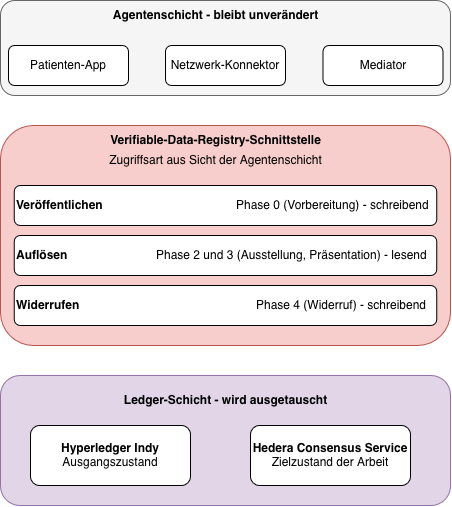
\includegraphics[width=\textwidth]{Figures/schichtenschnitt}
    \caption{Schnitt zwischen Agenten- und Ledger-Schicht mit den drei Berührungspunkten der Schnittstelle. Die Phasen entsprechen dem Credential-Lebenszyklus aus dem Abschnitt~\ref{sec:grundlagen-beispiel}; Phase 1 (Verbindung) kommt ohne Ledger-Zugriff aus und erscheint deshalb nicht.}
    \label{fig:schichtenschnitt}
\end{figure}

\subsection{Funktionen der Ledger-Schicht}
\label{subsec:ledger-funktionen}

Aus der Aufgabenzuweisung der Referenzarchitektur~\cite{erler2023} ergeben sich drei operative Funktionen der Ledger-Schicht: das öffentliche Verzeichnis der DIDs, die Verwaltung von Schemas und Credential Definitions sowie die Revocation Registry. Sie dienen einem übergeordneten Zweck, den Erler et al.\ der Blockchain ausdrücklich zuweisen -- sie soll als zusätzlicher Vertrauensanker wirken~\cite{erler2023} --, der hier als eigenständige Funktion geführt wird, da er in einer alternativen Implementierung eigene Mechanismen erfordert. Hinzu kommt die manipulationsresistente Transaktionshistorie, die Erler et al.\ nicht eigens benennen, die aber als Eigenschaft der Ledger-Technologie die Vertrauensanker-Funktion trägt~\cite{torongo2023}. Es ergeben sich damit fünf Kernfunktionen:

\begin{enumerate}
  \item \textbf{Vertrauensanker (Trust Anchor):} Der Ledger dient als zusätzlicher Vertrauensanker für die Netzwerkteilnehmer, indem er verifizierte digitale Identitäten institutioneller Teilnehmer öffentlich verankert~\cite{erler2023}. In Hyperledger Indy wird dies durch eine Vertrauenshierarchie implementiert, in der berechtigte Akteure (Stewards, Endorser) neue Teilnehmer per NYM-Transaktion registrieren, die eine DID, den entsprechenden Verifikationsschlüssel (Verkey) und die Rolle des Teilnehmers auf dem Ledger verankert~\cite{torongo2023}.
  \item \textbf{DID-Registry:} Der Ledger dient als öffentliches Verzeichnis der DIDs institutioneller Teilnehmer. Andere Teilnehmer können diese DIDs zu DID-Dokumenten konvertieren, um verifizierte Agent-zu-Agent-Verbindungen zu erstellen~\cite{erler2023}.
  \item \textbf{Schema- und Credential-Definition-Speicher:} Die Referenzarchitektur speichert Datenmodelle (Schemas) und Credential Definitions für die Ausstellung und Prüfung digital signierter Credentials auf dem Ledger~\cite{erler2023}. In Indy enthalten Schemas Name, Version und Attribute; Credential Definitions definieren darauf aufbauend Signaturtyp und Aussteller, und Verifier greifen bei der Prüfung lesend auf diese Objekte zu~\cite{torongo2023}.
  \item \textbf{Revocation Registry:} Die Referenzarchitektur enthält eine Revocation Registry zum Widerruf der Gültigkeit ausgestellter Credentials~\cite{erler2023}. In Indy wird dies auf Basis von kryptografischen Akkumulatoren geführt; Verifier prüfen vor der Anerkennung eines Credentials dessen Nicht-Widerrufsstatus gegen die Registry~\cite{torongo2023}.
  \item \textbf{Manipulationsresistente Transaktionshistorie:} Alle Schreiboperationen werden als kryptografisch verkettete Transaktionen gespeichert. Dadurch entsteht eine nachvollziehbare, manipulationsresistente Historie aller Änderungen an Identitäts- und Credentials-Metadaten, die als Audit-Grundlage dient~\cite{torongo2023} und damit die Vertrauensanker-Funktion der Referenzarchitektur stützt~\cite{erler2023}.
\end{enumerate}

Wie im Abschnitt~\ref{sec:grundlagen-speichermodelle} beschrieben, implementiert Indy diese Funktionen als native, direkt abfragbare Objekttypen des Domain Ledgers und wirkt damit nicht nur als Ordnungsdienst, sondern auch als Zustandsspeicher mit integrierter Lese-Semantik ~\cite{torongo2023, indynode}. Diese Eigenschaft ist für die spätere Abbildung auf den Hedera Consensus Service wichtig, da dieser ausschließlich Ordnung und Zeitstempelung von Nachrichten gewährleistet. Inhaltlich geht es bei den Schemas, Credential Definitions und Revocation-Einträgen um die im Abschnitt~\ref{subsec:grundlagen-anoncreds} eingeführten AnonCreds-Objekttypen, die Indy als native Ledger-Objekte umsetzt~\cite{anoncredsspec, torongo2023}. Diese Unterscheidung zwischen dem Credential-Format und seinem Speicherort ist die Voraussetzung des in dieser Arbeit vorgenommenen Austauschs: Da AnonCreds den Speicherort über die Abstraktion einer Verifiable Data Registry (Abschnitt~\ref{subsec:grundlagen-vdr}) offen lässt~\cite{anoncredsspec}, muss eine alternative Ledger-Schicht nicht das kryptographische Protokoll, sondern ausschließlich die Auflösung dieser Objekte neu implementieren. Die Tabelle~\ref{tab:ledger-funktionen-indy} fasst die Zuordnung der Funktionen zu den Indy-Mechanismen nach~\cite{torongo2023} zusammen. Diese Bindung an das bestehende Format ist gleichzeitig wichtig für den weiteren Entwurf: ein Wechsel auf ein anderes Credential-Format, z.B. das W3C-Verifiable-Credentials-Datenmodell~\cite{w3cvcdm}, steht nicht zur Auswahl, da die Aries-Protokolle zur Ausstellung und Prüfung an das AnonCreds-Format gebunden sind und eine Änderung damit FA6 sowie die im Abschnitt~\ref{subsec:abgrenzung} festgelegte Abgrenzung verletzen würde. Dasselbe gilt für den Widerrufsmechanismus: \texttt{RevRegDef} und \texttt{RevRegEntry} sind native, an das Akkumulatorverfahren gebundene AnonCreds-Objekttypen, gegen die der Nicht-Widerrufsnachweis als Bestandteil des Zero-Knowledge-Proofs geführt wird~\cite{anoncredsspec}. Alternative Verfahren - z.B. die Abbildung des Widerrufs als eigene Zustandstransaktion, wie sie Mamoru et al. umsetzen~\cite{mamoru2026} - würden das Present-Proof-Protokoll der Agenten verändern und stehen daher ebenfalls nicht zur Auswahl.


\begin{table}[htbp]
\renewcommand{\arraystretch}{1.3}
  \centering
  \caption{Funktionen der Ledger-Schicht und ihre Realisierung in
  Hyperledger Indy}
  \label{tab:ledger-funktionen-indy}
  \begin{tabular}{p{0.35\textwidth} p{0.55\textwidth}}
    \toprule
    \textbf{Ledger-Funktion} & \textbf{Mechanismus in Hyperledger
    Indy} \\
    \midrule
    Trust Anchor &
    NYM-Transaktionen mit Rollenzuweisung (Steward, Endorser) auf
    dem Domain Ledger \\
    DID-Registry &
    Öffentliche DIDs mit Verkeys als abfragbare Objekte des Domain
    Ledgers \\
    Schema-/Credential-Definition-Speicher &
    Schemas und Credential Definitions als native Objekttypen des
    Domain Ledgers \\
    Revocation Registry &
    Kryptografische Akkumulatoren mit Revocation-Registry-Einträgen
    auf dem Domain Ledger \\
    Manipulationsresistente Historie &
    Kryptografisch verkettete Transaktionslogs, konsensbasiert
    repliziert über RBFT (Plenum) \\
    \bottomrule
  \end{tabular}
\end{table}

\subsection{Abgrenzung des Austauschumfangs}
\label{subsec:abgrenzung}

Der in dieser Arbeit entwickelte Proof-of-Concept ersetzt nur die beschriebene Ledger-Schicht durch eine Alternative, die auf dem Hedera Consensus Service basiert. Alle Komponenten der Agenten-Schicht (Abschnitt~\ref{subsec:schichtenstruktur}) bleiben unverändert. Diese Abgrenzung folgt zwei Gedanken. Erstens berühren paarweise Peer-DIDs den Ledger konzeptionell nicht, sodass die Agentenschicht von einem Austausch der Ledger-Schicht funktional unabhängig ist~\cite{erler2023}. Zweitens stellt die Konsistenz aller anderen Komponenten sicher, dass die bei der späteren Evaluation gemessenen Unterschiede entlang Performanz, Skalierbarkeit und Sicherheit auf die Ledger-Schicht zugeordnet werden können und nicht durch Änderungen an anderen Architekturbausteinen verfälscht werden.

\section{Anforderungen}
\label{sec:konzipierung-anforderungen}
Die Analyse der Referenzarchitektur im Abschnitt~\ref{sec:konzipierung-referenzarchitektur} sowie die im Kapitel~\ref{cha:state_of_the_art} abgeleitete Vergleichskriterien bestimmen Anforderungen an die zu konzipierende HCS-basierte Ledger-Schicht. Anforderungen sind in funktionale und nicht-funktionale Anforderungen unterteilt. Die funktionalen Anforderungen ergeben sich direkt aus der Aussage der funktionalen Äquivalenz: Der Proof-of-Concept ersetzt die Ledger-Schicht, ohne die Agenten-Schicht zu verändern, und muss daher dieselben fünf Kernfunktionen bereitstellen, die im Abschnitt~\ref{subsec:ledger-funktionen} definiert sind. Die nicht-funktionalen Anforderungen beschreiben die drei Evaluationsdimensionen dieser Arbeit - Performanz, Skalierbarkeit und Sicherheit - und bilden somit die Grundlage für das spätere Evaluationskonzept. Es sollte betont werden, dass sich alle Anforderungen auf die zu ersetzende Ledger-Schicht beziehen und nicht auf das Gesamtsystem; Anforderungen an die Komponenten, die unverändert übernommen wurden, wurden von Erler et al. im Rahmen des Threat-Modeling-Prozesses der Referenzarchitektur berücksichtigt~\cite{erler2023}.


\subsection{Funktionale Anforderungen}
\label{subsec:funktionale-anforderungen}
\begin{description}
  \item[FA1 - Autorisierung von Schreiboperationen über eine Vertrauenshierarchie:] Die Ledger-Schicht muss die Vertrauensanker-Funktion erfüllen, die ihr die Referenzarchitektur zuweist~\cite{erler2023}, indem sie schreibende Operationen auf autorisierte Akteure beschränkt und dabei mindestens zwei Berechtigungsstufen unterscheidet: eine Wurzel, die neue autorisierte Akteure aufnimmt, und eine delegierte Stufe, die daraufhin eigene Schreiboperationen durchführen darf. In Hyperledger Indy wird diese Hierarchie über die Rollen Steward und Endorser implementiert und vom Ledger selbst umgesetzt~\cite{torongo2023}.
  \item[FA2 - Verwaltung und Auflösung öffentlicher DIDs:] Die Ledger-Schicht muss öffentliche DIDs institutioneller Teilnehmer verwalten und zu DID-Dokumenten mit zugehörigem Verifikationsschlüssel auflösen, sodass Agenten verifizierte Verbindungen aufbauen können~\cite{erler2023}. Neben der Erzeugung und der Auflösung muss sie dabei auch die Aktualisierung eines DID-Dokuments (u.a. die Rotation des Verifikationsschlüssels) sowie die Deaktivierung einer DID unterstützen, da diese Operationen Bestandteil des DID-Lebenszyklus sind~\cite{mazzocca2025} und in Indy über NYM-Transaktionen ebenfalls zur Verfügung stehen~\cite{torongo2023}.
  \item[FA3 - Verwaltung von Schemas und Credential Definitions:] Die Ledger-Schicht muss die Veröffentlichung und den lesenden Abruf von Schemas und Credential Definitions ermöglichen, wie es die Referenzarchitektur für die Ausstellung und Prüfung von Credentials vorsieht~\cite{erler2023}. Die abgerufenen Objekte müssen dabei dem AnonCreds-Datenmodell entsprechen~\cite{anoncredsspec}, da die Agentenschicht unverändert bleibt.
  \item[FA4 - Widerruf von Credentials:] Die Ledger-Schicht muss die Veröffentlichung von Widerrufsinformationen sowie die Prüfung des Nicht-Widerrufsstatus unterstützen, entsprechend der Revocation Registry der Referenzarchitektur~\cite{erler2023}. Da der Nicht-Widerrufsnachweis in AnonCreds als Bestandteil des Zero-Knowledge-Proofs gegen den kryptografischen Akkumulator geführt wird~\cite{anoncredsspec}, muss der jeweils aktuelle Zustand dieses Akkumulators öffentlich abrufbar sein.
  \item[FA5 - Manipulationsresistente, nachvollziehbare Historie:] Alle Schreiboperationen auf der Ledger-Schicht müssen in einer kryptografisch gesicherten, zeitlich geordneten und nachträglich nicht unbemerkt veränderbaren Historie erfasst werden, die als Audit-Grundlage dienen kann. Die Anforderung umfasst dabei zwei Eigenschaften: die Integrität der Historie und ihre dauerhafte Abrufbarkeit. Diese Unterscheidung ist notwendig, weil beide Eigenschaften je nach Ledger-Technologie von derselben oder von unterschiedlichen Komponenten erbracht werden (Abschnitt~\ref{sec:grundlagen-speichermodelle}).
  \item[FA6 - Kompatibilität zur Agentenschicht:] Die Ledger-Schicht muss ihre Funktionen über Schnittstellen bereitstellen, die von der unverändert übernommenen Aries-Agentenschicht verwendet werden können, ohne dass Änderungen an den DIDComm-Protokollen, den Peer-DID-Mechanismen oder den Protokollen zur Ausstellung und Präsentation von Credentials benötigt werden. Diese Anforderung folgt direkt aus der im Abschnitt~\ref{subsec:abgrenzung} festgelegten Abgrenzung und ist gleichzeitig die Voraussetzung dafür, dass gemessene Unterschiede der Ledger-Schicht zugeordnet werden können.
\end{description}

\subsection{Nicht-funktionale Anforderungen}
\label{subsec:nichtfunktionale-anforderungen}

Die nicht-funktionalen Anforderungen entsprechen eins zu eins den sieben in Kapitel~\ref{cha:state_of_the_art} hergeleiteten Vergleichskriterien (Tabelle~\ref{tab:synthese_vergleichskriterien}). Sie formulieren bewusst keine Schwellenwerte, da deren Messung und Vergleich gerade das empirische Ziel dieser Arbeit sind; stattdessen beschreibt jede Anforderung, welche strukturelle Eigenschaft die zu entwerfende Architektur unterstützen muss, damit sie entlang des jeweiligen Kriteriums überhaupt messbar ist. Die Ausgestaltung der Messung selbst ist Gegenstand des Evaluationskonzepts.


\begin{description}
  \item[NFA1 - Durchsatz:] Die Ledger-Schicht muss jede Schreiboperation (z.B. Registrierungs-, Schema-, Credential-Definition- und Widerrufsoperationen) so ausführen, dass ihre Annahme, ihre Ablehnung und ihr Abschluss für die einreichende Komponente eindeutig unterscheidbar sind. Nur dadurch lässt sich unter identischer Last bestimmen, wie viele Operationen je Zeiteinheit tatsächlich wirksam werden und ab welcher Rate Operationen abgewiesen werden.
  \item[NFA2 - Latenz:] Die Ledger-Schicht muss für jede der im Abschnitt~\ref{subsec:ledger-funktionen} identifizierten Kernfunktionen einen beobachtbaren, klar definierten Zeitpunkt der Finalität bereitstellen, der nach Operationstyp differenziert ist, sodass operationsspezifische Latenzen zwischen Indy und HCS vergleichbar gemessen werden können. Da lesende Zugriffe im Lebenszyklus eines Credentials deutlich häufiger auftreten als schreibende (Tabelle~\ref{tab:beispiel-ledgerzugriffe}), muss dies für Lese- und Schreiboperationen genau so gelten.
  \item[NFA3 - Ressourcenverbrauch:] Die an der Ledger-Schicht beteiligten Client- und Infrastrukturkomponenten müssen ihren CPU- und Speicherverbrauch während der Evaluation beobachtbar und den einzelnen Ledger-Funktionen zuordenbar machen. Der Entwurf muss dazu offenlegen, welche Komponenten für die Erbringung der Ledger-Funktionen betrieben werden müssen, damit der Vergleich beide Varianten in ihrem jeweils vollständigen Umfang erfasst.
  \item[NFA4 - Lastskalierung:] Die Ledger-Schicht darf keine strukturellen Obergrenzen für die Anzahl der Teilnehmer, der verwalteten Identitätsobjekte oder der parallel eingereichten Operationen enthalten, die den Messbereich vor Erreichen der technologiebedingten Grenze beschränken. Zusätzlich muss der Entwurf die Komponenten benennen, an denen ein Engpass auftreten kann, sodass beobachtete Veränderungen von Durchsatz und Latenz einer konkreten Komponente zugeordnet werden können.
  \item[NFA5 - Datenwachstum:] Die Ledger-Schicht muss den mit wachsendem Datenbestand verbundenen Speicherbedarf auf Ledger- und Knoten-Ebene nachvollziehbar und quantifizierbar machen, sodass das Datenwachstum der gewählten Zustandsrekonstruktionsstrategie mit dem nativen Zustandsspeicher von Indy verglichen werden kann.
  \item[NFA6 - Konsens-Fehlertoleranz:] Die Ledger-Schicht muss so betrieben werden können, dass Anzahl, Verteilung und Konfiguration der konsensbildenden Knoten kontrollierbar sind und einzelne Knoten gezielt ausgefallen oder fehlerhaft betrieben werden können. Nur unter dieser Bedingung lassen sich das aBFT-Modell des Hedera-Hashgraph-Konsens und das RBFT-Modell von Indy-Plenum unter vergleichbaren Knotenkonfigurationen entlang byzantinischer Fehlertoleranz und Finalitätsgarantien vergleichen, statt Eigenschaften zweier unterschiedlich dimensionierter Netzwerke gegenüberzustellen.
  \item[NFA7 - Zugriffskontrolle und Widerruf:] Die Ledger-Schicht muss die Wirksamkeit der in FA1 geforderten Autorisierung und des in FA4 geforderten Widerrufsmechanismus auswertbar machen: Der Versuch einer nicht autorisierten Schreiboperation muss ein beobachtbares, eindeutiges Ergebnis liefern, und der Widerrufsstatus eines Credentials muss so veröffentlicht werden, dass ein Verifier ihn eindeutig gegen den aktuellen Akkumulatorzustand auswerten kann. Nur unter dieser Bedingung lassen sich beide Mechanismen überhaupt gegen die Referenzarchitektur vergleichen, statt sie nur konzeptionell zu behaupten.
\end{description}

Die funktionalen und nicht-funktionalen Anforderungen bilden zusammen den Bewertungsmaßstab für die im folgenden Abschnitt entwickelten Entwurfsentscheidungen: Jede dort getroffene Entscheidung wird explizit gegen die hier formulierten Anforderungen abgewogen.

\section{Entwurf}
\label{sec:konzipierung-entwurf}

Basierend auf den im Abschnitt~\ref{sec:konzipierung-anforderungen} beschriebenen funktionalen und nicht-funktionalen Anforderungen werden im Folgenden die Entwurfsentscheidungen für die HCS-basierte Ledger-Schicht getroffen. Jede Entscheidung wird nach demselben Schema behandelt: zuerst wird das Problem beschrieben, das aus der Differenz zwischen Hyperledger Indy und dem Hedera Consensus Service stammt; anschließend werden die möglichen Optionen vorgestellt, wobei jeweils offengelegt wird, woraus sich die betrachtete Option ergibt - aus der Literatur des Kapitels~\ref{cha:state_of_the_art}, aus den Spezifikationen oder aus der Vollständigkeit der von HCS bereitgestellten Mechanismen. Die Optionen werden anschließend gegen die Anforderungen aus dem Abschnitt~\ref{sec:konzipierung-anforderungen} bewertet, bevor die getroffene Entscheidung begründet wird.

Die Entscheidungen sind nicht unabhängig voneinander, sondern bauen in einer festen Reihenfolge aufeinander auf. Die Entscheidungen E1 bis E6 betreffen den Entwurf der Ledger-Schicht selbst: E1 definiert, auf welchem Netzwerk sie betrieben wird und welche Eigenschaften dadurch netzwerkseitig garantiert sind; E2 bestimmt, in welcher Form die Identitätsobjekte überhaupt auf dem Ledger abgelegt werden, und schränkt damit ein, welche Methoden für die einzelnen Objekttypen zur Auswahl stehen; E3 und E4 wählen diese Methoden für öffentliche DIDs bzw. für die AnonCreds-Objekte; E5 legt fest, wie aus dem geordneten Nachrichtenstrom ein lesbarer Zustand entsteht; E6 ergänzt die Vertrauenshierarchie, die weder das Netzwerk noch die gewählten Methoden abdecken. Die abschließende Entscheidung E7 betrifft nicht den Entwurf der Ledger-Schicht, sondern ihre Anbindung an die unverändert übernommene Agentenschicht und wird deshalb zuletzt getroffen und gegen E3 bis E5 auf Widerspruchsfreiheit geprüft.


\subsection{Grundproblem: Zustands-Ledger gegenüber Ordnungsdienst}
\label{subsec:grundproblem-state-vs-ordering}

Der in Abschnitt~\ref{sec:grundlagen-speichermodelle} dargestellte Unterschied der beiden Speichermodelle liegt allen folgenden Entwurfsentscheidungen zugrunde. Er wird deshalb zuerst in drei Schritten behandelt: ob er für die Aufgabenstellung dieser Arbeit überhaupt ein Problem darstellt, mit welchen Strategien die betrachtete Literatur ihm begegnet und welche dieser Strategien hier gewählt wird.

\paragraph{Ist die fehlende Zustandshaltung ein Problem?}
Die fehlende Zustandshaltung ist keine Unvollständigkeit von HCS, sondern eine Entwurfseigenschaft: Der Dienst trennt die Ordnung von Nachrichten von ihrer Auswertung und überlässt letztere den abonnierenden Anwendungen~\cite{bairdgross2019}. Ob daraus ein Problem entsteht, hängt deshalb nicht von der Technologie ab, sondern davon, welche Funktionen von ihr erwartet werden. Gemessen an den fünf im Abschnitt~\ref{subsec:ledger-funktionen} identifizierten Ledger-Funktionen ergibt sich ein differenziertes Bild. Für die manipulationsresistente Historie (Funktion 5) entsteht kein Problem, da Ordnung, Konsens-Zeitstempel und Integritätssicherung genau die Leistung sind, die HCS nativ erbringt. Für die Vertrauensanker-Funktion (Funktion 1) entsteht ein Teilproblem, da HCS über den \texttt{submitKey} zwar zwischen berechtigt und unberechtigt unterscheidet, aber kein Rollenkonzept kennt. Ein vollständiges Problem entsteht bei den drei Funktionen, die ein adressierbares Objekt voraussetzen - DID-Registry, Schema- und Credential-Definition-Speicher sowie Revocation Registry (Funktionen 2 bis 4) -, denn die Agentenschicht fragt dort nicht nach einer Nachricht, sondern nach dem aktuellen Stand eines Objekts. Drei der fünf Funktionen müssen deshalb auf der Anwendungsebene reproduziert werden, eine teilweise und eine gar nicht.

\paragraph{Wie adressiert die betrachtete Literatur diesen Unterschied?}
Aus den im Kapitel~\ref{cha:state_of_the_art} betrachteten Arbeiten und den einschlägigen Spezifikationen lassen sich fünf Strategien unterscheiden, mit denen der Ort der Zustandshaltung festgelegt wird (Tabelle~\ref{tab:zustandsstrategien}); sie schließen einander nicht aus, sondern werden in einzelnen Arbeiten je Objektklasse unterschiedlich kombiniert. Für die vorliegende Arbeit sind daran zwei Beobachtungen wesentlich. Erstens beantworten die meisten Arbeiten des Korpus die Frage gar nicht, weil sie mit Hyperledger Indy, Hyperledger Fabric oder Ethereum Plattformen einsetzen, die den Zustand selbst führen; die Frage stellt sich überhaupt erst beim Wechsel auf einen reinen Ordnungsdienst. Zweitens umgeht die einzige hashgraphbasierte Architektur des Gesundheitskontexts das Problem, statt es zu lösen: Verma et al. verzichten auf ein dezentrales Identitätsmodell und benötigen deshalb keine ledger-adressierbaren Identitätsobjekte~\cite{verma2024}. Damit ist die Frage, wie die Zustandshaltung für eine SSI-basierte Architektur auf einem reinen Ordnungsdienst gelöst wird, in der betrachteten Gesundheitsliteratur nicht beantwortet; belegte Antworten liefern allein die Spezifikationen und die ergänzende Literatur außerhalb des Gesundheitskontexts~\cite{bairdgross2019, hasheddidmethod, satybaldy2026}. Dies konkretisiert die im Abschnitt~\ref{sec:literatur_schlussfolgerungen} formulierte Forschungslücke auf der Entwurfsebene.

\begin{table}[htbp]
\renewcommand{\arraystretch}{1.3}
\footnotesize
  \centering
  \caption{Strategien der Zustandshaltung in der betrachteten Literatur}
  \label{tab:zustandsstrategien}
  \begin{tabular}{p{0.17\textwidth} p{0.43\textwidth} p{0.26\textwidth}}
    \toprule
    \textbf{Strategie} & \textbf{Mechanismus} & \textbf{Vertreter} \\
    \midrule
    Zustand im Ledger & Der Ledger führt typisierte Objekte und beantwortet Leseanfragen selbst; für die Anwendung stellt sich die Frage nicht & \cite{torongo2023, manoj2022, tawfik2025, joshimahajan2025} \\
    Zustand in der Anwendung & Die Anwendung abonniert den Nachrichtenstrom dauerhaft und schreibt den daraus abgeleiteten Zustand lokal fort (Appnet-Muster) & \cite{bairdgross2019} \\
    Zustand in einem externen Speicher & Das Objekt liegt off-chain, auf dem Ledger wird nur ein Hashwert oder Verweis verankert & \cite{mazlan2020, farin2025, tawfik2025, mamoru2026, guptaverma2026} \\
    Rekonstruktion je Zugriff & Der Zustand wird bei jedem Lesezugriff aus der Historie des betreffenden Topics abgeleitet; vorgehalten wird nichts & \cite{hasheddidmethod, satybaldy2026} \\
    Vermeidung & Die Architektur verzichtet auf ledger-adressierbare Identitätsobjekte und benötigt deshalb keinen Zustand auf dem Ledger & \cite{verma2024} \\
    \bottomrule
  \end{tabular}
\end{table}
\normalsize

\paragraph{Lösungsweg dieser Arbeit.}
Die Strategie der Vermeidung steht nicht zur Auswahl, da die Referenzarchitektur ein SSI-basiertes Identitätsmodell voraussetzt~\cite{erler2023} und die Agentenschicht nach FA6 unverändert bleibt. Die verbleibenden drei Strategien werden in den folgenden Entscheidungen gegen die Anforderungen bewertet und dabei auf zwei Teilfragen aufgeteilt: Die Entscheidung E2 legt fest, in welcher Form die Objekte überhaupt auf den Ledger geschrieben werden, und wägt dazu die Auslagerung in einen externen Speicher gegen die vollständige Kodierung ab. Die Entscheidung E5 legt fest, wie aus dem geordneten Nachrichtenstrom wieder ein lesbares Objekt entsteht, und wägt dazu die Zustandshaltung in der Anwendung gegen die Rekonstruktion je Zugriff ab. Die Entscheidung E6 ergänzt das Teilproblem der Vertrauensanker-Funktion, für das keine der fünf Strategien eine Antwort liefert. Der Ort der Zustandshaltung ist damit nicht eine, sondern drei Entscheidungen, die im Abschnitt~\ref{sec:konzipierung-zielarchitektur} zusammengeführt werden.

\subsection{E1 - Netzwerkbetriebsmodell und Vertrauensgrenze}
\label{subsec:e1-netzwerkmodell}

\paragraph{Problem.}
Der Netzwerktyp einer DLT wird über drei unabhängig ausprägbare Eigenschaften beschrieben~\cite{erler2024}: den Betrieb der konsensbildenden Knoten (permissionless, permissioned oder als Konsortium mehrerer gleichberechtigter Organisationen), den Schreibzugang und den Lesezugang. Das Attribut öffentlich bezeichnet in dieser Arbeit ausschließlich die dritte Eigenschaft. Referenzarchitektur und öffentliches Hedera-Netzwerk unterscheiden sich entlang dieser Achsen weniger, als die gebräuchlichen Sammelbezeichnungen nahelegen: Beide betreiben ein permissioned Konsensnetzwerk mit öffentlichem Lesezugang~\cite{erler2023, bairdharmon2019}. Der Unterschied liegt darin, wer die Knotenmenge stellt und ob ihre Zusammensetzung für die beteiligten Institutionen bestimmbar ist -- in der Referenzarchitektur betreiben die Institutionen die Validatorknoten selbst, und die Steward-Rolle ist zugleich eine Rolle im Konsens~\cite{erler2023, torongo2023}.

\paragraph{Optionen.}
Die erste Option ist der Betrieb auf dem öffentlichen Hedera-Netzwerk. Verma et al. wählen diesen Weg für ihre hashgraphbasierte Architektur zur Verwaltung elektronischer Patientenakten; sie bezeichnen ihr Netzwerk zwar als permissioned, betreiben ihre Anwendung jedoch auf dem öffentlichen Hedera-Netzwerk, dessen Lesezugriff öffentlich ist~\cite{verma2024}. Die zweite Option ist der Betrieb eines selbst kontrollierten Hashgraph-Netzwerks. Cádiz et al. verankern W3C-konforme DIDs und Verifiable Credentials auf einem permissioned Teegraph-Ledger, dessen Knoten von den beteiligten Akteuren selbst betrieben werden~\cite{cadiz2025}. Für die Hedera-Software existiert diese Möglichkeit ebenfalls in Form lokal betreibbarer Netzwerkinstanzen~\cite{hederanetworks}.

\paragraph{Bewertung.}
Die Optionen unterscheiden sich darin, wer die Konsensknoten betreibt, und damit in drei für diese Arbeit relevanten Punkten.

Erstens die Fehlertoleranz nach NFA6. Das öffentliche Hedera-Netzwerk erreicht seine aBFT-Eigenschaften über eine vom Governing Council betriebene Knotenmenge, deren Größe und Zusammensetzung ein Nutzer weder kennt noch beeinflusst~\cite{bairdharmon2019}. NFA6 verlangt dagegen, Anzahl, Verteilung und Konfiguration der Knoten kontrollieren und einzelne Knoten gezielt fehlerhaft betreiben zu können; das erfüllt allein ein selbst betriebenes Netzwerk. Daraus folgt zugleich eine Randbedingung: Eine Instanz mit einem einzigen Knoten genügt nicht, da sie die zu vergleichende Eigenschaft gar nicht ausprägt.

Zweitens die Vergleichbarkeit der Messung nach NFA1, NFA2 und NFA4. Ein Vergleich zwischen einem lokal betriebenen Indy-Netzwerk und dem öffentlichen Hedera-Netzwerk würde Unterschiede messen, die auf Netzwerkgröße, geografische Verteilung, Fremdlast und Transaktionsgebühren zurückgehen, statt auf die Ledger-Technologie -- und damit der in Abschnitt~\ref{subsec:abgrenzung} formulierten Zuordenbarkeit widersprechen.

Drittens die Sichtbarkeit der abgelegten Objekte. Hier ist eine Abgrenzung nötig, um die Wirkung dieser Entscheidung nicht zu überschätzen: Wer auf ein Topic schreiben darf, entscheidet in beiden Optionen nicht das Konsensnetzwerk, sondern die in Abschnitt~\ref{subsec:e6-vertrauenshierarchie} behandelten Mechanismen. Die Netzwerkwahl verändert dagegen, wer die Historie lesen kann: Auf dem öffentlichen Netzwerk ist der Nachrichtenstrom jedes Topics über öffentliche Mirror Nodes für beliebige Dritte abrufbar, wodurch die abgelegten Identitätsmetadaten offengelegt werden~\cite{satybaldy2026}; in einem selbst betriebenen Netzwerk bleibt der Lesezugriff auf das Konsortium beschränkt. Da die Referenzarchitektur sicherheitsgetrieben entworfen wurde~\cite{erler2023}, ist diese Verengung der Vertrauensgrenze der näher liegende Entwurf.

Die Entscheidung betrifft damit nicht permissioned gegenüber permissionless -- beide Optionen sind permissioned --, sondern die Kontrolle über die Knotenmenge und den Lesezugang.

\paragraph{Entscheidung.}
Die HCS-basierte Ledger-Schicht wird auf einem selbst betriebenen Hashgraph-Netzwerk konzipiert, dessen Konsensknoten unter der Kontrolle der beteiligten Institutionen stehen. Damit bleibt die Vertrauensgrenze der Referenzarchitektur erhalten und beide Ledger-Varianten können unter vergleichbaren Bedingungen gemessen werden. Aus dieser Entscheidung folgen zwei Randbedingungen für die Umsetzung, die im Kapitel~\ref{cha:implementierung} eingelöst werden: Die ausgewählte Netzwerkinstanz muss mit mehreren Knoten betreibbar sein, und sie muss eine selbst betriebene Mirror Node umfassen, da im öffentlichen Netzwerk bereitgestellte Mirror Nodes den Nachrichtenstrom eines privaten Netzwerks nicht ausliefern. Die Mirror Node wird damit zum Bestandteil der Ledger-Schicht und geht in die Systemgrenze der Messung nach NFA3 ein.


\subsection{E2 - Speicherform der Identitätsobjekte}
\label{subsec:e2-speicherform}

\paragraph{Problem.}
Da HCS keinen Zustand speichert, muss definiert werden, was als Nachricht auf den Ledger geschrieben wird. Für die Gesundheitsdaten ist dies bereits entschieden: Sie bleiben off-chain~\cite{erler2023} und sind nach Abschnitt~\ref{subsec:abgrenzung} nicht Gegenstand des Austauschs. Offen ist die Frage für die vier Objektgruppen der Ledger-Schicht -- öffentliche DIDs, Schemas, Credential Definitions und Widerrufsinformationen. Bei Indy stellt sie sich nicht, da der Domain Ledger sie als native Objekttypen hält (Abschnitt~\ref{subsec:grundlagen-speicher-indy}). Auf HCS entsteht sie, weil eine Nachricht auf 1024 Byte begrenzt ist (Abschnitt~\ref{subsec:grundlagen-speicher-hcs}), während Credential Definitions und Revocation Registry Definitions diese Grenze deutlich überschreiten; die Hiero AnonCreds Method dokumentiert ein Beispiel, in dem eine CredDef auf sechs und eine RevRegDef auf zwei Nachrichten aufgeteilt werden~\cite{hieroanoncreds}, wobei die Nachrichtenzahl mit der Attributenzahl des Schemas wächst.

\paragraph{Optionen.}
Der Optionsraum ergibt sich aus drei Speichermustern der Literatur und der HCS-Spezifikationen.

Die erste Option ist die vollständige Kodierung jeder Zustandsänderung als Nachricht, aus der Anwendungen den Zustand durch Replay des geordneten Stroms rekonstruieren. Baird et al.\ beschreiben dies als Appnet-Modell~\cite{bairdgross2019}: Die Konsensknoten ordnen, zeitstempeln und verwerfen die Nachrichten, während Mirror Nodes und abonnierende Mitglieder die Historie behalten und den Zustand lokal ableiten. Die Hedera-DID-Methode wendet das Muster an und definiert die Auflösung als Verarbeitung der Nachrichten in Konsensreihenfolge~\cite{hasheddidmethod}.

Die zweite Option ist das Hash-Anchoring, bei dem das Objekt außerhalb des Ledgers liegt und nur ein Hashwert konstanter Größe verankert wird. Mazlan et al.\ beschreiben es als generische Speicheroptimierung~\cite{mazlan2020}; in den untersuchten Umsetzungen ist es das dominierende Muster~\cite{farin2025, tawfik2025, mamoru2026}.

\paragraph{Bewertung.}
Erler et al.~\cite{erler2023} nennen für die Ledger-Schicht genau vier Objektgruppen: öffentliche DIDs als dezentrale Public-Key-Infrastruktur, Schemas, Credential Definitions und eine Revocation Registry. Die Gesundheitsdaten selbst liegen off-chain~\cite{erler2023}. Zu entscheiden ist allein, in welcher Form diese vier Gruppen auf HCS abgelegt werden.

Für das Hash-Anchoring spricht nur das Größenproblem -- es ersetzt ein mehrteiliges Objekt durch einen Verweis konstanter Größe. Genau dieses Problem löst jedoch bereits die dritte Option innerhalb des Ledgers, da HCS-1 die Aufteilung und Wiederzusammensetzung größerer Objekte standardisiert~\cite{hcs1standard}; die Motivation entfällt damit, die Nachteile bleiben. Hinzu kommt, dass die SSI-basierten Arbeiten für Identitätsmetadaten umgekehrt verfahren und sie vollständig auf dem Ledger ablegen, da dort ausschließlich öffentlich sichtbare und keine personenbezogenen Objekte liegen~\cite{torongo2023,manoj2022}.

Den Ausschlag geben drei Anforderungen. FA3 und FA4 verlangen den Abruf von Schemas, Credential Definitions und Akkumulatorzustand in einer dem AnonCreds-Datenmodell entsprechenden Form~\cite{anoncredsspec}; beim Hash-Anchoring läge dieses Objekt nicht auf dem Ledger, sondern in einem externen Speicher, dessen Auflösung zusätzlich zu definieren wäre. FA5 fordert eine dauerhaft abrufbare, manipulationsresistente Historie; das Hash-Anchoring sichert jedoch nur den Hashwert, während Verfügbarkeit und Integrität des referenzierten Objekts außerhalb des Konsenses liegen. Die vollständige Kodierung entspricht dagegen allen drei Anforderungen unmittelbar und liefert nach Satybaldy et al. zudem die niedrigste gemessene Auflösungslatenz aller untersuchten DID-Methoden~\cite{satybaldy2026}.

\paragraph{Entscheidung.}
Die vollständige Objektkodierung auf dem Ledger wird ausgewählt; das Hash-Anchoring wird verworfen. In welcher der beiden Kodierungsformen (einzelne Topic-Nachricht oder HCS-1-Datei) ein Objekt jeweils gespeichert wird, ist keine eigenständige Entscheidung, sondern ergibt sich aus den in E3 und E4 gewählten Methoden.


\subsection{E3 - Wahl der DID-Methode}
\label{subsec:e3-did-methode}

\paragraph{Problem.}
FA2 erfordert die Verwaltung öffentlicher DIDs institutioneller Teilnehmer einschließlich ihrer Aktualisierung und Deaktivierung sowie deren Auflösung zu DID-Dokumenten mit zugehörigem Verifikationsschlüssel. Indy verwendet dafür seine eigene Ledger-DID-Methode; für die HCS-basierte Alternative muss eine DID-Methode ausgewählt werden.

\paragraph{Optionen.}
Der Optionsraum ist hier durch die Fragestellung dieser Arbeit bereits weitgehend definiert und wird deshalb kürzer als die übrigen Entscheidungen betrachtet. Da HCS als Ledger ausgewählt ist, entfallen die ledgerbasierten Methoden anderer Plattformen; die von Satybaldy et al. im selben Vergleich untersuchten Methoden \texttt{did:ethr} und \texttt{did:xrpl}~\cite{satybaldy2026} setzen jeweils einen anderen Ledger voraus und stehen daher nicht zur Auswahl. Es verbleiben zwei Klassen beschriebener Methoden. Erstens die ledgerlosen Methoden, für die \texttt{did:key} steht: Der Identifikator wird vollständig aus dem Schlüsselmaterial abgeleitet, das DID-Dokument bei Bedarf lokal erzeugt, und die Spezifikation sieht weder eine öffentliche Registrierung noch eine Aktualisierung oder Deaktivierung vor~\cite{didkeyspec}. Zweitens die HCS-gestützte Methode \texttt{did:hedera}, bei der Änderungen am DID-Dokument als Nachrichten auf einem HCS-Topic veröffentlicht werden und die Topic-ID Bestandteil des Identifikators ist, sodass die Auflösung über Mirror Nodes öffentlich möglich ist~\cite{hasheddidmethod}.

\paragraph{Bewertung.}
\texttt{did:key} erfüllt FA2 in mehrfacher Hinsicht nicht: Die Methode kennt keine öffentliche Registrierung, und da der Identifikator aus dem Schlüssel abgeleitet ist, sind weder eine Schlüsselrotation noch eine Deaktivierung vorgesehen~\cite{didkeyspec}. Damit kann sie weder die Vertrauensanker-Funktion der Ledger-Schicht übernehmen noch den in FA2 geforderten DID-Lebenszyklus abbilden. Es verbleibt \texttt{did:hedera}, was gleichzeitig dem Muster der SSI-basierten Arbeiten entspricht, die DID-Methode vom eingesetzten Ledger zu beziehen: Torongo und Toorani~\cite{torongo2023} sowie Manoj et al.~\cite{manoj2022} nutzen Indy-Verinyms für öffentliche Identitäten und paarweise Peer-DIDs für die Kommunikation; Manoj et al. begründen die Vermeidung einer smart-contract-basierten Identitätsverwaltung damit, dass die Verknüpfung eines Identifikators an einen Smart Contract dessen unabhängige Existenz aufhebt und die Identität den Sicherheitsproblemen des Contracts aussetzt~\cite{manoj2022}. Umsetzungen, die zwar W3C-konforme DIDs verwenden, das zugehörige Schlüsselmaterial aber von einer Middleware erzeugen und verwahren lassen~\cite{farin2025} oder in einer hardwaregestützten Trusted Execution Environment halten~\cite{cadiz2025}, verlagern die Schlüsselkontrolle vom Inhaber auf den Betreiber bzw. auf die Hardware und widersprechen damit dem nutzerzentrierten Ansatz, den die Referenzarchitektur für das Identitätsmanagement vorsieht~\cite{erler2023}. Satybaldy et al. begründen die verbleibende Option zusätzlich empirisch: Im direkten Vergleich weist \texttt{did:hedera} unter den drei untersuchten Methoden die geringste Latenz für Ledger-Operationen und gleichzeitig die geringste Metadaten-Offenlegung auf~\cite{satybaldy2026}.

\paragraph{Entscheidung.}
Es wird die Methode \texttt{did:hedera} verwendet. Für die folgenden Entscheidungen sind zwei Konsequenzen festzuhalten. Erstens legt die Methode für jede öffentliche DID ein eigenes Topic an, da die Topic-ID Bestandteil des Identifikators ist, und gibt damit einen Teil der Topic-Struktur der Ledger-Schicht bereits vor~\cite{hasheddidmethod}. Zweitens werden Änderungen am DID-Dokument als einzelne Topic-Nachrichten und nicht als HCS-1-Datei kodiert; für den Objekttyp der öffentlichen DIDs ist die in E2 offengelassene Kodierungsfrage damit beantwortet.


\subsection{E4 - Abbildung der AnonCreds-Objekte}
\label{subsec:e4-anoncreds-abbildung}

\paragraph{Problem.}
FA3 und FA4 verlangen, dass Schemas, Credential Definitions und Widerrufsinformationen im AnonCreds-Datenmodell veröffentlicht und abgerufen werden können. Der Abschnitt~\ref{subsec:ledger-funktionen} hat festgehalten, dass Indy diese Objekte als native Transaktionstypen des Domain Ledgers führt und dass AnonCreds den Speicherort über die Abstraktion einer Verifiable Data Registry offen lässt~\cite{anoncredsspec}. Für HCS muss daher definiert werden, wie die vier AnonCreds-Objekttypen auf Topics und Nachrichten abgebildet und wie ihre Identifikatoren gebildet werden.

\paragraph{Optionen.}
Die erste Option ist eine für diese Arbeit eigens entworfene Abbildung, die die Objekte nach einem selbst definierten Schema auf Topics verteilt. Sie ist aus den in E2 gewählten Mechanismen direkt konstruierbar, da HCS-1 die Ablage beliebiger unveränderlicher Objekte definiert~\cite{hcs1standard}.

Die zweite Option ist die Hiero AnonCreds Method, eine bereits spezifizierte Registry-Methode für AnonCreds auf Hedera. Sie publiziert Schema, Credential Definition und Revocation-Registry-Definition jeweils als eigene HCS-1-Datei mit eigenem Topic sowie die zugehörigen Registry-Einträge auf einem weiteren, der Registry-Definition zugeordneten Topic~\cite{hieroanoncreds}; die zugrunde liegende Festlegung von HCS als Verifiable Data Registry für AnonCreds ist als Hedera Improvement Proposal dokumentiert~\cite{hip762}.

Nicht zur Auswahl steht dagegen ein Wechsel des Widerrufsmechanismus - etwa auf statuslistenbasierte Verfahren nach dem W3C-Modell~\cite{bitstringstatuslist} oder auf eine Abbildung des Widerrufs als eigene Zustandstransaktion, wie sie Mamoru et al. umsetzen~\cite{mamoru2026}. Der Abschnitt~\ref{subsec:ledger-funktionen} hat bereits festgehalten, dass der Nicht-Widerrufsnachweis in AnonCreds Bestandteil des Zero-Knowledge-Proofs ist und eine Änderung des Verfahrens das Present-Proof-Protokoll der Agenten und damit FA6 verletzen würde.

\paragraph{Bewertung.}
Beide Optionen erfüllen FA3 und FA4 grundsätzlich, unterscheiden sich jedoch in ihrem Verhältnis zu FA6. Eine eigene Abbildung müsste auf der Seite der Agentenschicht durch eine ebenfalls eigens entwickelte Registry-Implementierung ergänzt werden; die Kompatibilität zur unveränderten Agentenschicht wäre dann nicht durch eine Spezifikation, sondern durch die eigene Implementierung zu belegen. Die Hiero AnonCreds Method definiert dagegen sowohl die Ablage als auch die Bildung der Objektidentifikatoren, sodass die Auflösung eines Objekts allein aus seinem Identifikator möglich ist~\cite{hieroanoncreds} - genau die Eigenschaft, die Indy über seine nativen Objekttypen bereitstellt (Abschnitt~\ref{subsec:grundlagen-speicher-indy}) und die die Agentenschicht bei der Prüfung einer Präsentation voraussetzt.

Dazu kommt ein methodisches Argument. Das Ziel dieser Arbeit ist der Vergleich zweier Ledger-Technologien, nicht der Vergleich einer etablierten Implementierung mit einem Eigenentwurf. Eine selbst definierte Abbildung würde in die Messung Eigenschaften der eigenen Implementierung einbringen, die sich nicht von den Eigenschaften des Ledgers trennen lassen, und damit der im Abschnitt~\ref{subsec:abgrenzung} formulierten Zuordenbarkeit widersprechen. Eine spezifizierte Methode verschiebt diesen Anteil auf eine dokumentierte, von Dritten geprüfte Grundlage.

\paragraph{Entscheidung.}
Die AnonCreds-Objekte werden nach der Hiero AnonCreds Method abgebildet~\cite{hieroanoncreds}; ein eigener Abbildungsentwurf wird verworfen. Für die Kodierungsfrage aus E2 folgt daraus, dass Schema, Credential Definition und Revocation-Registry-Definition als HCS-1-Dateien und die Revocation-Registry-Einträge als Nachrichten eines zugeordneten Topics gespeichert werden. Der Widerrufsmechanismus von AnonCreds (der kryptografische Akkumulator) bleibt unverändert; ausgetauscht wird ausschließlich der Ort, an dem sein Zustand veröffentlicht wird. Die Tabelle~\ref{tab:anoncreds-kodierung-hcs} fasst die Kodierung je Objekttyp zusammen und nimmt die in E3 getroffene Festlegung für die öffentlichen DIDs mit auf.


\begin{table}[htbp]
\renewcommand{\arraystretch}{1.3}
\footnotesize
  \centering
  \caption{Kodierung der AnonCreds-Objekte auf HCS nach der Hiero AnonCreds Method}
  \label{tab:anoncreds-kodierung-hcs}
  \begin{tabular}{p{0.20\textwidth} p{0.20\textwidth} p{0.50\textwidth}}
    \toprule
    \textbf{Objekt} & \textbf{Kodierung} & \textbf{Begründung} \\
    \midrule
    Schema & HCS-1-Datei & Statisches, einmalig publiziertes Objekt; eigenes Topic je Objekt~\cite{hieroanoncreds} \\
    CredDef & HCS-1-Datei & Statisches, einmalig publiziertes Objekt; überschreitet die 1024-Byte-Grenze einer einzelnen Nachricht deutlich, wobei die Zahl der benötigten Nachrichten mit der Attributzahl des zugrunde liegenden Schemas wächst - im Beispiel der Spezifikation sechs Chunks~\cite{hieroanoncreds} \\
    RevRegDef & HCS-1-Datei & Statisches, einmalig publiziertes Objekt; enthält zusätzlich den Verweis auf das Entries-Topic (\texttt{hcsMetadata.entriesTopicId}); im Beispiel der Spezifikation auf zwei Chunks aufgeteilt~\cite{hieroanoncreds} \\
    RevRegEntry & Einzelne HCS-Nachricht & Wiederkehrende, inkrementelle Aktualisierung; enthält nur das komprimierte Delta (geänderte Indizes und Akkumulator) seit dem letzten Eintrag, veröffentlicht im der RevRegDef zugeordneten Entries-Topic~\cite{hieroanoncreds} \\
    Öffentliche DID (\texttt{did:hedera}) & Einzelne HCS-Nachricht je Änderung & Wiederkehrende, inkrementelle Aktualisierung; DID-Dokument wird aus dem Nachrichtenstrom des DID-eigenen Topics rekonstruiert~\cite{hasheddidmethod} \\
    \bottomrule
  \end{tabular}
\end{table}
\normalsize

\subsection{E5 - Leseweg und Materialisierung des Zustands}
\label{subsec:e5-leseweg}

\paragraph{Problem.}
Die Entscheidungen E2 bis E4 legen fest, was auf den Ledger geschrieben wird. Damit ist jedoch noch nicht bestimmt, wie ein Verifier ein Objekt wieder liest. Bei Indy ist das eine Protokolloperation gegen den Zustandsspeicher der Validatorknoten (Abschnitt~\ref{subsec:grundlagen-speicher-indy}); bei HCS existiert keine solche Operation, sondern nur der über eine Mirror Node abrufbare Nachrichtenstrom eines Topics~\cite{bairdgross2019}. Diese Entscheidung ist für die Evaluation besonders wichtig: die Tabelle~\ref{tab:beispiel-ledgerzugriffe} zeigt, dass eine einzelne Präsentationsprüfung auf vier Objekte lesend zugreift, sodass der Leseweg die nach NFA2 gemessene Latenz stärker prägt als jede Schreiboperation.

\paragraph{Optionen.}
Der Optionsraum ergibt sich aus den beiden Zugriffsarten, die eine Mirror Node bereitstellt. Die erste Option ist die Auflösung je Lesezugriff: die auswertende Komponente ruft bei jeder Anfrage die Historie des betreffenden Topics ab und leitet den aktuellen Zustand des Objekts direkt daraus ab. Sie hält selbst keinen Zustand. Die zweite Option ist das von Baird et al. beschriebene Appnet-Muster: die Komponente abonniert den Nachrichtenstrom der relevanten Topics dauerhaft, führt den daraus abgeleiteten Zustand lokal fort und beantwortet Lesezugriffe aus diesem lokalen Zustand~\cite{bairdgross2019}.

\paragraph{Bewertung.}
Für NFA2 unterscheiden sich die Optionen grundlegend. Bei Auflösung je Lesezugriff wächst der Aufwand mit der Länge der Topic-Historie, da der Zustand jedes Mal neu abgeleitet wird; bei fortgeschriebenem lokalem Zustand ist der Lesezugriff davon unabhängig, und der Aufwand verlagert sich auf die laufende Fortschreibung. Satybaldy et al. führen die von ihnen gemessene niedrige Latenz gerade darauf zurück, dass die Historie eines Topics isoliert ausgewertet werden kann~\cite{satybaldy2026} -- für die nach NFA5 zu untersuchende Entwicklung bei wachsendem Bestand ist jedoch genau die Abhängigkeit von der Historienlänge der interessierende Effekt. Für FA5 ist maßgeblich, dass die Konsensknoten den Nachrichteninhalt nach der Ordnung verwerfen~\cite{bairdgross2019}: Beide Optionen setzen deshalb eine Mirror Node voraus, die damit keine externe Infrastruktur ist, sondern Teil der gemessenen Systemgrenze und der erste Kandidat für den nach NFA4 zu lokalisierenden Engpass.

Den Ausschlag geben drei Punkte. Erstens bleibt die Agentenschicht nach FA6 unverändert, und die Lesezugriffe entstehen ausschließlich innerhalb dieser Schicht; eine zusätzliche Zustandskomponente stünde nicht auf dem tatsächlichen Lesepfad, sondern neben ihm und führte einen in der Referenzarchitektur nicht vorgesehenen zweiten Zugriffsweg ein. Zweitens ist die Abhängigkeit der Lesedauer von der Historienlänge genau der Unterschied zwischen Zustandsspeicher und Ordnungsdienst, den diese Arbeit messen soll; ein fortgeschriebener Zustand beseitigte diesen Effekt, bevor er quantifiziert ist, und das Ergebnis wäre keine Eigenschaft der Technologie mehr, sondern der eigenen Optimierung. Drittens wäre eine nur auf der HCS-Seite eingeführte Zustandskomponente kein symmetrischer Versuchsaufbau, da die Indy-Variante unverändert und ohne Zwischenspeicher betrieben wird.

\paragraph{Entscheidung.}
Es wird kein Zustand vorgehalten; jeder Lesezugriff wird durch Abruf und Auswertung der Topic-Historie über die Mirror Node beantwortet. Der lokal fortgeschriebene Zustand nach dem Appnet-Muster wird als Alternative verworfen, bleibt jedoch als Optimierungsmöglichkeit dokumentiert und wird in Abschnitt~\ref{sec:results-grenzen} anhand der gemessenen Werte eingeordnet. Der so festgelegte Leseweg ist damit ausdrücklich eine bewusst nicht optimierte Referenzkonfiguration: Er bildet den Zugriffsweg ab, den die Ledger-Technologie ohne zusätzliche anwendungsseitige Mittel bereitstellt, und nicht die bestmöglich erreichbare Konfiguration; die berichteten Lesewerte sind entsprechend als obere Schranke des Aufwands und nicht als Leistungsgrenze von HCS zu lesen (Abschnitt~\ref{subsec:eval-validitaet}). Für die Evaluation folgt daraus, dass die Länge der Topic-Historie ein bewusst zu setzender Versuchsparameter und kein Nebeneffekt ist: Der zu messende Zusammenhang zwischen Datenbestand und Lesedauer wird nur sichtbar, wenn die Bestände hinreichend groß gewählt werden (Abschnitt~\ref{sec:konzipierung-evaluationskonzept}). Die Mirror Node und die von ihr vorgehaltene Historie bilden zusammen mit dem Konsensnetzwerk und dem Registry-Adapter die Ledger-Schicht im Sinne der Messung.


\subsection{E6 - Vertrauenshierarchie, Schreibberechtigung und Topic-Struktur}
\label{subsec:e6-vertrauenshierarchie}

\paragraph{Problem.}
FA1 erfordert eine Vertrauenshierarchie mit mindestens zwei Berechtigungsstufen, in der nur autorisierte Akteure schreiben dürfen. In Indy definiert der Ledger diese Hierarchie selbst: Nur Akteure mit entsprechender Rolle können gültige NYM-Transaktionen einreichen~\cite{torongo2023}. HCS kennt keine rollenbasierte Schreibberechtigung. Zu entscheiden ist zunächst, über welchen Mechanismus die Hierarchie umgesetzt wird; davon abhängig ist der zweite Teil, auf welcher Topic-Struktur sie geführt wird. Der zweite Teil betrifft ausschließlich die Vertrauenshierarchie selbst, da die Topics der DID-Registry sowie der AnonCreds-Objekte durch die in E3 und E4 gewählten Methoden bereits vorgegeben sind~\cite{hasheddidmethod,hieroanoncreds}.

\paragraph{Optionen.}
Der Optionsraum für den Mechanismus lässt sich nicht aus der Literatur ableiten, da keine der untersuchten Arbeiten eine Vertrauenshierarchie auf HCS umsetzt; er ergibt sich aus den beiden von den Spezifikationen dokumentierten Kontrollpunkten. Der erste ist der netzwerkseitige \texttt{submitKey} eines Topics: Ist er gesetzt, akzeptiert das Netzwerk nur entsprechend signierte Nachrichten. Er kann auch als Threshold Key ausgeprägt sein, bei dem die Signatur von $N$ aus $M$ hinterlegten Schlüsseln genügt, sodass sich die Schreibberechtigung als Schwellenregel mehrerer Instanzen ausdrücken lässt (Abschnitt~\ref{subsec:grundlagen-hedera-plattform}). Der zweite Kontrollpunkt ist die anwendungsseitige Prüfung im Appnet-Modell, bei der die auswertende Anwendung Nachrichten ohne gültigen Rollennachweis beim Aufbau ihres lokalen Zustands verwirft~\cite{bairdgross2019}. Aus der Kombination beider ergibt sich eine dritte Möglichkeit. Für die Topic-Struktur liefern die Fabric-basierten Arbeiten beide Extreme -- ein einziger Kanal für das gesamte Netzwerk~\cite{joshimahajan2025} gegenüber vier nach Funktion getrennten Teil-Ledgern~\cite{tawfik2025} --, sodass ein gemeinsames Topic oder eine Aufteilung auf mehrere zur Wahl stehen.

\paragraph{Bewertung.}
Die Literatur zeigt für die inhaltliche Ausgestaltung der Hierarchie ein durchgehendes Muster: eine netzwerkseitig verankerte Wurzel mit einer delegierten zweiten Stufe. Bei Torongo und Toorani nimmt der Steward neue Akteure auf und vergibt die Rollen Trust Anchor bzw.\ Endorser, wobei ein Governance-Gremium darüber entscheidet, wer Steward wird~\cite{torongo2023}; Manoj et al.\ weisen diese Wurzel institutionell dem Gesundheitsministerium zu~\cite{manoj2022}. Dasselbe Muster findet sich in den Fabric-basierten Arbeiten unter anderer Bezeichnung~\cite{joshimahajan2025,tawfik2025}.

Da die Wurzel demnach keine Eigenschaft eines einzelnen Akteurs ist, sondern eines Gremiums, bildet ein Threshold Key als \texttt{submitKey} sie am genauesten ab: Er überträgt das kollektive Entscheiden mehrerer Instanzen unmittelbar auf den Signaturmechanismus und wird netzwerkseitig durchgesetzt. Die delegierte zweite Stufe lässt sich damit jedoch nicht ausdrücken, da der \texttt{submitKey} nur zwischen berechtigt und unberechtigt unterscheidet und keine Rollen kennt. Eine rein anwendungsseitige Prüfung wiederum gäbe die netzwerkseitige Verankerung der Wurzel auf, womit die geforderte Vertrauensanker-Funktion~\cite{erler2023} allein von der korrekten Implementierung der Leseseite abhinge. Die Kombination beider Kontrollpunkte bildet das belegte zweistufige Muster am genauesten ab und erfüllt FA1 und NFA7 am vollständigsten, da beide Stufen ein beobachtbares Ergebnis liefern: Eine unberechtigte Nachricht wird entweder vom Netzwerk abgewiesen oder von der auswertenden Komponente verworfen.

Zwei Punkte bleiben dabei offen und werden in der Entscheidung festgelegt. Auf der Wurzelstufe ist jede Änderung des Steward-Kreises zugleich eine Änderung des Topics selbst und nur mit dem \texttt{adminKey} möglich (Abschnitt~\ref{subsec:grundlagen-hcs-topics}): Bleibt dieser ungesetzt, ist der Kreis dauerhaft eingefroren; wird er als einzelner Schlüssel gesetzt, kann dessen Inhaber die Schwellenregel aushebeln. Auf der zweiten Stufe sind die Topics der öffentlichen DIDs und der AnonCreds-Objekte zwar objektgebunden schlüsselgeschützt, doch prüft das Netzwerk nur den Besitz des objekteigenen Schlüssels und nicht den Delegationsstatus seines Inhabers. Die auswertende Komponente benötigt deshalb zwei Angaben, die aus den Kontrollpunkten selbst nicht folgen: ein Merkmal, an dem sie eine Nachricht ihrem Schreiber zuordnet, und eine zeitliche Bezugsgröße, gegen die sie den Delegationszustand prüft.

Für die Topic-Struktur geben die gewählten Methoden bereits vor, dass \texttt{did:hedera} je öffentlicher DID ein Topic anlegt~\cite{hasheddidmethod} und die Hiero AnonCreds Method die AnonCreds-Objekte ebenfalls auf mehrere Topics verteilt~\cite{hieroanoncreds}. Die Ledger-Schicht besteht damit aus einer wachsenden Zahl kleiner, unabhängiger Topics. Daraus folgt eine für FA5 wesentliche Einschränkung: HCS garantiert eine Totalordnung ausschließlich innerhalb eines Topics~\cite{bairdgross2019}, sodass eine übergreifende Historie nachträglich aus den Konsens-Zeitstempeln rekonstruiert werden muss.

\paragraph{Entscheidung.}
Die Vertrauenshierarchie wird auf einem einzelnen Topic geführt, dessen \texttt{submitKey} als Threshold Key von den Steward-Instanzen gemeinsam kontrolliert wird; der \texttt{adminKey} erhält dieselbe Schwellenregel, damit der Steward-Kreis änderbar bleibt, ohne dass eine einzelne Instanz die Wurzel übernehmen kann. Ob die Regel im Versuchsaufbau mit mehreren oder einem Schlüssel besetzt wird, ist für die gemessenen Eigenschaften ohne Belang und wird in Kapitel~\ref{cha:implementierung} festgelegt.

Endorser-Rechte werden über Delegationsnachrichten auf demselben Topic vergeben und entzogen. Da der \texttt{submitKey} den Schreibzugriff auf den Steward-Kreis beschränkt, ist ihre Herkunft bereits durch die Annahme der Nachricht belegt, und die Hierarchie umfasst genau die von FA1 geforderten zwei Stufen, weil Endorser weder sich selbst entziehen noch weiter delegieren können. Die Gültigkeit prüft der Registry-Adapter als auswertende Komponente des in E5 festgelegten Lesewegs, indem er die Historie des Vertrauens-Topics bei jeder Prüfung erneut ausliest -- und zwar gegen den Delegationszustand zum Konsens-Zeitstempel der bewerteten Objektnachricht, sodass ein späterer Entzug bereits geschriebene Objekte nicht rückwirkend entwertet und das Verhalten dem von Indy entspricht~\cite{torongo2023}. Welches Merkmal der durch E3 und E4 vorgegebenen Nachrichtenformate die Zuordnung einer Nachricht zu ihrem Schreiber trägt, ist eine Eigenschaft der gewählten Methoden und wird in Kapitel~\ref{cha:implementierung} festgestellt; ist der Delegationszustand nicht lesbar, gilt die Nachricht als ungültig. Die in FA5 geforderte topicübergreifende Historie wird aus den Konsens-Zeitstempeln der beteiligten Topics rekonstruiert; der Aufwand geht in die Messung nach NFA2 ein und wäre nach NFA3 gesondert zu erfassen.

Die anwendungsseitige Prüfstufe dieses Entwurfs setzt eine Komponente voraus, die von der unveränderten Agentenschicht nicht bereitgestellt wird und die diese Arbeit selbst hätte implementieren müssen. Eine solche Komponente würde nicht die verglichene Ledger-Technologie, sondern eine eigene, im Rahmen dieser Arbeit entstandene Erweiterung messen, deren Aussagekraft für den Vergleich zwischen Indy und HCS grundsätzlich anders zu bewerten wäre als die native Rollenprüfung des Indy-Ledgers. Diese anwendungsseitige Stufe wird daher, wie die in Abschnitt~\ref{subsec:e5-leseweg} verworfene Alternative des lokal fortgeschriebenen Zustands, als Optimierungspotenzial dokumentiert und nicht als Bestandteil der Zielarchitektur umgesetzt (Abschnitt~\ref{sec:results-grenzen}). Das Szenario S5 prüft entsprechend die netzwerkseitige Stufe auf beiden Varianten vollständig und die Widerrufs-Auswertbarkeit nach FA4, nicht die anwendungsseitige Delegation auf der HCS-Variante.

\subsection{E7 - Anbindung an die Agentenschicht}
\label{subsec:e7-agentenanbindung}

\paragraph{Problem.}
FA6 verlangt, dass die Aries-Agentenschicht die entworfene Ledger-Schicht ohne Änderung ihrer Protokolle verwenden kann. Die Agenten der Referenzarchitektur sprechen jedoch die Indy-eigenen Lese- und Schreiboperationen an (Abschnitt~\ref{subsec:grundlagen-speicher-indy}), die HCS nicht kennt. Zu entscheiden ist daher, über welche Komponente die in E2 bis E6 entworfene Ledger-Schicht an die unveränderte Agentenschicht angebunden wird.

\paragraph{Optionen.}
Der Optionsraum wird durch die im Abschnitt~\ref{subsec:ledger-funktionen} beschriebene Abstraktion der Verifiable Data Registry (Abschnitt~\ref{subsec:grundlagen-vdr}) eröffnet: AnonCreds trennt das kryptografische Protokoll vom Speicherort und definiert die Registry als austauschbare Schnittstelle~\cite{anoncredsspec}. Die erste Option ist eine im Rahmen dieser Arbeit entwickelte Registry- und Resolver-Implementierung, die diese Schnittstelle gegen die in E3 bis E5 festgelegten Mechanismen bedient. Die zweite Option ist die Verwendung einer bestehenden Erweiterung des Agentenframeworks: Für Aries Cloud Agent Python existiert ein Hedera-Plugin, das \texttt{did:hedera} auflöst und AnonCreds-Objekte über HCS bereitstellt~\cite{acapyhedera}.

\paragraph{Bewertung.}
Beide Optionen lassen die DIDComm- und Peer-DID-Mechanismen unberührt, da diese nach Abschnitt~\ref{subsec:schichtenstruktur} den Ledger konzeptionell nicht berühren. Sie unterscheiden sich in zwei Punkten.

Erstens in der Belastbarkeit des Nachweises für FA6. Eine eigene Implementierung belegt die Kompatibilität nur für den eigenen Aufbau; eine bestehende Erweiterung des Frameworks belegt sie für die reguläre Erweiterungsschnittstelle des Agenten und macht damit sichtbar, dass der Austausch der Ledger-Schicht keine Änderung an den Protokollen erfordert.

Zweitens ist die Zuordenbarkeit der Messergebnisse nach Abschnitt~\ref{subsec:abgrenzung}. Eine eigene Implementierung würde Eigenschaften einbringen, die sich in der Messung nicht von den Eigenschaften des Ledgers trennen lassen. Dasselbe methodische Argument war bereits für E4 entscheidend.

Zu prüfen bleibt die Widerspruchsfreiheit gegenüber E3 bis E5. Die bestehende Erweiterung setzt \texttt{did:hedera} und die Hiero AnonCreds Method um~\cite{acapyhedera,hasheddidmethod,hieroanoncreds} und ist damit mit E3 und E4 konsistent. Für E5 besteht die Konsistenz darin, dass das Plugin selbst keinen Zustand vorhält, sondern den Stand eines Objekts bei jedem Lesezugriff aus der über die Mirror Node abgerufenen Topic-Historie ableitet und damit genau den in E5 gewählten Leseweg realisiert. Da dies eine Eigenschaft des Plugins und keine Festlegung der Spezifikation ist, wird sie im Rahmen der Implementierung überprüft und dokumentiert; von ihr hängt die Interpretation der nach NFA2 und NFA5 gemessenen Lesevorgänge ab.

\paragraph{Entscheidung.}
Die Anbindung erfolgt über das bestehende Hedera-Plugin des Agentenframeworks~\cite{acapyhedera}; eine eigene Registry-Implementierung wird verworfen. Die Agentenschicht bleibt damit unverändert, und der Austausch beschränkt sich auf die Registry-Schnittstelle unterhalb der Aries-Protokolle. Der von der Erweiterung realisierte Leseweg wird im Kapitel~\ref{cha:implementierung} gegen die Festlegung aus E5 geprüft; eine Abweichung wäre kein Widerspruch zum Entwurf, muss aber bei der Auswertung nach NFA2 und NFA5 offengelegt werden.


\subsection{Überblick}
\label{subsec:entwurf-ueberblick}

Die Tabelle~\ref{tab:entwurfsentscheidungen} fasst die sieben Entwurfsentscheidungen mit der jeweils gewählten Option und den dadurch adressierten Anforderungen zusammen. Jede der in Abschnitt~\ref{sec:konzipierung-anforderungen} formulierten Anforderungen wird dabei von mindestens einer Entscheidung getragen.

\begin{table}[htbp]
\renewcommand{\arraystretch}{1.3}
\footnotesize
  \centering
  \caption{Entwurfsentscheidungen der HCS-basierten Ledger-Schicht im Überblick}
  \label{tab:entwurfsentscheidungen}
  \begin{tabular}{p{0.19\textwidth} p{0.44\textwidth} p{0.24\textwidth}}
    \toprule
    \textbf{Entscheidung} & \textbf{Gewählte Option} & \textbf{Adressierte Anforderungen} \\
    \midrule
    E1 - Netzwerkbetriebsmodell und Vertrauensgrenze & Selbst betriebenes, mehrknotiges Hashgraph-Netzwerk mit eigener Mirror Node unter Kontrolle der beteiligten Institutionen & NFA6; Vergleichbarkeit der Messung (NFA1, NFA2, NFA4) \\
    E2 - Speicherform der Identitätsobjekte & Vollständige Kodierung der Identitätsobjekte auf dem Ledger & FA3, FA4, FA5; NFA5 \\
    E3 - Wahl der DID-Methode & \texttt{did:hedera} mit einem eigenen Topic je öffentlicher DID & FA2; NFA2 \\
    E4 - Abbildung der AnonCreds-Objekte & Hiero AnonCreds Method; unveränderter akkumulatorbasierter Widerrufsmechanismus & FA3, FA4, FA6; NFA1, NFA5 \\
    E5 - Leseweg und Materialisierung des Zustands & Auflösung je Lesezugriff über die Mirror Node; lokal fortgeschriebener Zustand nach dem Appnet-Muster als begründet verworfene Alternative & FA5; NFA2, NFA5 \\
        E6 - Vertrauenshierarchie, Schreibberechtigung und Topic-Struktur & Ein einzelnes Vertrauens-Topic; Wurzel netzwerkseitig über einen Threshold Key als \texttt{submitKey}, \texttt{adminKey} unter derselben Schwellenregel; delegierte Endorser-Stufe über Delegationsnachrichten mit anwendungsseitiger Prüfung als Entwurf, dessen Umsetzung im Kapitel~\ref{cha:implementierung} als Optimierungspotenzial statt als realisierte Komponente geführt wird & FA1, FA5; NFA7 \\
    E7 - Anbindung an die Agentenschicht & Bestehendes Hedera-Plugin des Aries-Agentenframeworks über die Verifiable-Data-Registry-Schnittstelle von AnonCreds & FA6; NFA2, NFA3, NFA5 \\
    \bottomrule
  \end{tabular}
\end{table}
\normalsize

Die getroffenen Entscheidungen betreffen jeweils einen Teilaspekt der Ledger-Schicht. Der folgende Abschnitt führt sie zu einer Gesamtarchitektur zusammen und zeigt, wie die fünf im Abschnitt~\ref{subsec:ledger-funktionen} identifizierten Ledger-Funktionen im Zusammenspiel der Komponenten erbracht werden.

\section{Zielarchitektur}
\label{sec:konzipierung-zielarchitektur}

Die Entscheidungen E1 bis E7 ergeben zusammen die Zielarchitektur der HCS-basierten Ledger-Schicht. Dieser Abschnitt fasst sie zusammen: zuerst die beteiligten Komponenten und anschließend die Abbildung der fünf Ledger-Funktionen aus Abschnitt~\ref{subsec:ledger-funktionen} auf HCS-Mechanismen.

\subsection{Komponenten}
\label{subsec:zielarchitektur-komponenten}

\begin{description}
  \item[Konsensnetzwerk:] Mehrknotiges, selbst betriebenes Hashgraph-Netzwerk; erbringt Ordnung, Konsens-Zeitstempel und Finalität (E1). Die konkrete Umsetzung wird im Kapitel~\ref{cha:implementierung} festgelegt.
  \item[Mirror Node:] Selbst betrieben; hält die Nachrichtenhistorie dauerhaft vor und stellt Abfrage- und Abonnementschnittstelle bereit~\cite{hederamirrornodes} (E1, E5).
  \item[Topics:] Ein Vertrauens-Topic für Registrierungs- und Delegationsnachrichten (E6), je ein Topic pro öffentlicher DID~\cite{hasheddidmethod} (E3) sowie die Topics der AnonCreds-Objekte nach der Hiero AnonCreds Method~\cite{hieroanoncreds} (E4).
  \item[Registry-Adapter:] Bildet die Lese- und Schreiboperationen der Verifiable-Data-Registry-Schnittstelle von AnonCreds auf Topic-Operationen ab und leitet den Zustand eines Objekts bei jedem Lesezugriff aus der über die Mirror Node abgerufenen Historie ab (E5, E7); dabei prüft er die Delegationskette gegen das Vertrauens-Topic (E6).
  \item[Agentenschicht:] Unverändert übernommen (Abschnitt~\ref{subsec:abgrenzung}); nicht Teil der Ledger-Schicht.
\end{description}

Für das Zusammenspiel dieser Komponenten ist eine Eigenschaft festzuhalten, die die HCS-basierte Variante von der Referenzvariante unterscheidet: Auf dem Schreibweg ist keine zustandsführende Komponente beteiligt. Das Netzwerk ordnet die Nachricht, versieht sie mit einem Konsens-Zeitstempel und stellt sie über die Mirror Node bereit. Eine netzwerkseitige Prüfung der Vertrauenshierarchie findet ausschließlich auf dem Vertrauens-Topic statt, dessen Schreibberechtigung nach E6 gesetzt ist; die Topics der öffentlichen DIDs und der AnonCreds-Objekte sind zwar ebenfalls schlüsselgeschützt, jedoch objektgebunden und unabhängig von dieser Hierarchie. Ob ein schreibender Akteur zum Zeitpunkt des Schreibens delegiert war, wird deshalb erst beim Lesen ausgewertet (E5). Der Aufwand des Lesewegs wächst dadurch mit der Länge der Topic-Historie - genau der Zusammenhang, den die Evaluation nach NFA2 und NFA5 quantifiziert; zugleich entsteht die Asymmetrie gegenüber Indy, das den unberechtigten Schreibvorgang bereits abweist, die das Szenario S5 untersucht.

\begin{figure}[htbp]
    \centering
    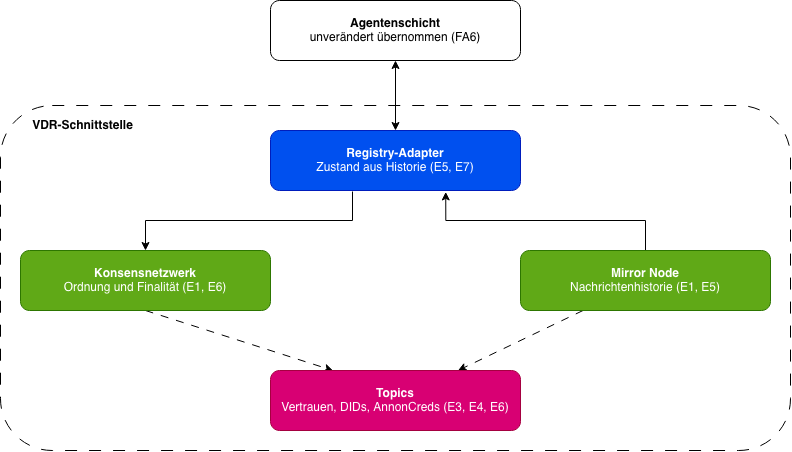
\includegraphics[width=\textwidth]{Figures/zielarchitektur}
    \caption{Zielarchitektur der HCS-basierten Ledger-Schicht mit Schreib- und Lesepfad. Die gestrichelte Linie markiert die Messgrenze an der Verifiable-Data-Registry-Schnittstelle.}
    \label{fig:zielarchitektur}
\end{figure}

Die Abbildung~\ref{fig:zielarchitektur} fasst die Topics zu einer Komponente zusammen, obwohl sie durch die Entscheidungen E3, E4 und E6 unterschiedlich strukturiert sind. Die Abbildung~\ref{fig:topic-struktur} differenziert sie nach ihrem Inhalt und ihrer Anzahl aus. Für die Evaluation ist daran eine Unterscheidung wesentlich: Von den sechs Topic-Typen wachsen drei über die Zeit - das Vertrauens-Topic mit jeder Änderung der Delegationsrechte (E6), die Topics der öffentlichen DIDs mit jeder Aktualisierung des DID-Dokuments, etwa bei einer Schlüsselrotation oder einer Deaktivierung nach FA2 (E3), und das Topic des Widerrufsstatus mit jedem Widerruf (E4). Die drei Topics der HCS-1-kodierten Objekte - Schema, Credential Definition und Widerrufsregister-Definition - bleiben nach ihrer Veröffentlichung unverändert. Da der in E5 festgelegte Leseweg nur bei den wachsenden Topics mit dem Bestand teurer wird, ist die Lesedauer nach NFA5 nicht für alle Objekttypen bestandsabhängig; das Szenario S3 sollte die drei wachsenden Typen deshalb getrennt erfassen. Inwieweit dies eingelöst werden konnte, weist Abschnitt~\ref{sec:results-s3} aus.

\begin{figure}[htbp]
    \centering
    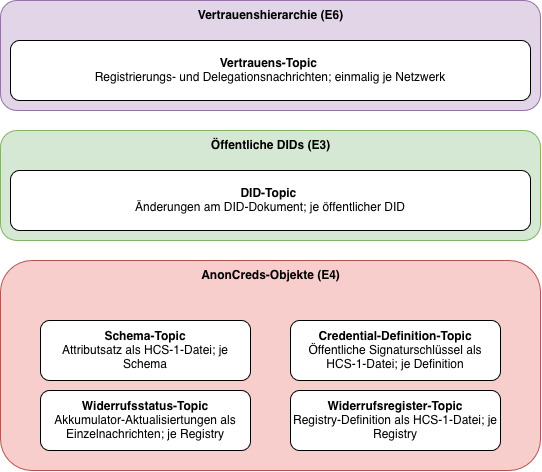
\includegraphics[width=\textwidth]{Figures/topic-struktur}
    \caption{Topic-Struktur der HCS-basierten Ledger-Schicht nach den Entwurfsentscheidungen E3, E4 und E6. Das Vertrauens-Topic ist das einzige Topic, dessen Schreibberechtigung an die Vertrauenshierarchie gebunden ist; alle übrigen Topics sind objektgebunden schlüsselgeschützt, aber unabhängig von dieser Hierarchie, die Auswertung der Berechtigung erfolgt beim Lesen.}
    \label{fig:topic-struktur}
\end{figure}


\subsection{Abbildung der Ledger-Funktionen}
\label{subsec:zielarchitektur-funktionsabbildung}

Die Tabelle~\ref{tab:ledger-funktionen-hcs} ist das Gegenstück zur Tabelle~\ref{tab:ledger-funktionen-indy} und ordnet jeder Kernfunktion den realisierenden Mechanismus sowie die zugrunde liegende Entwurfsentscheidung zu.

\begin{table}[htbp]
\renewcommand{\arraystretch}{1.3}
\footnotesize
  \centering
  \caption{Funktionen der Ledger-Schicht und ihre Realisierung in der HCS-basierten Variante}
  \label{tab:ledger-funktionen-hcs}
  \begin{tabular}{p{0.24\textwidth} p{0.52\textwidth} p{0.10\textwidth}}
    \toprule
    \textbf{Ledger-Funktion} & \textbf{Mechanismus in der HCS-basierten Variante} & \textbf{Entsch.} \\
    \midrule
    Trust Anchor & Threshold Key als \texttt{submitKey} des Vertrauens-Topics (Wurzel); Endorser-Stufe über signierte Delegationsnachrichten mit anwendungsseitiger Prüfung & E6 \\
    DID-Registry & \texttt{did:hedera}; DID-Dokument wird aus dem Nachrichtenstrom des DID-eigenen Topics rekonstruiert & E3, E5 \\
    Schema-/Credential-Definition-Speicher & Vollständige Kodierung der Objekte nach der Hiero AnonCreds Method; Ablage als HCS-1-Dateien & E2, E4 \\
    Revocation Registry & \texttt{RevRegDef} und \texttt{RevRegEntry} als Topic-Objekte; Akkumulatorzustand aus dem jüngsten Eintrag & E4 \\
    Manipulationsresistente Historie & Konsens-Zeitstempel und Ordnung des Hashgraph-Konsens; dauerhafte Abrufbarkeit über die selbst betriebene Mirror Node & E1, E5 \\
    \bottomrule
  \end{tabular}
\end{table}
\normalsize

\section{Evaluationskonzept}
\label{sec:konzipierung-evaluationskonzept}

Die Evaluation vergleicht die im Abschnitt~\ref{sec:konzipierung-zielarchitektur} entworfene HCS-basierte Ledger-Schicht differenziell mit der Indy-basierten Ledger-Schicht der Referenzarchitektur. Der Vergleich ist entlang der nicht-funktionalen Anforderungen NFA1 bis NFA7 organisiert, die ihrerseits eins zu eins den Vergleichskriterien aus Tabelle~\ref{tab:synthese_vergleichskriterien} entsprechen. Dieser Abschnitt legt fest, welche Größen gemessen werden, an welchen Punkten sie erhoben werden, unter welchen Szenarien gemessen wird, wie die Sicherheitsdimension bewertet wird und welche Grenzen für die Gültigkeit der Ergebnisse gelten. Die technische Umsetzung des Messaufbaus ist Gegenstand des Kapitels~\ref{cha:implementierung}, die Ergebnisdarstellung des Kapitels~\ref{sec:results}.

\subsection{Messgrößen und Messpunkte}
\label{subsec:eval-messgroessen}

Die Messgrößen werden nicht frei gewählt, sondern aus der in Kapitel~\ref{cha:state_of_the_art} ausgewerteten Literatur abgeleitet; die Messpunkte dagegen nicht, da die untersuchten Evaluationen unterschiedliche Systemgrenzen verwenden und gerade deshalb untereinander nicht vergleichbar sind (Abschnitt~\ref{sec:literatur_schlussfolgerungen}). Sie ergeben sich stattdessen aus der Zielarchitektur und werden im Anschluss an Tabelle~\ref{tab:messgroessen} festgelegt.

Für die Performanz sind Durchsatz und Latenz die in der Methodikliteratur ausgewiesenen Standardmetriken~\cite{sehimibendaoud2023} und werden in den benchmarkbasierten Evaluationen des Korpus durchgängig verwendet~\cite{tawfik2025, joshimahajan2025, chainarong2025}. Dass die Latenz nach Operationstyp differenziert wird, folgt Arbeiten, die je Lebenszyklusoperation messen~\cite{manoj2022, mamoru2026, satybaldy2026}; der Ressourcenverbrauch stammt aus Arbeiten, die CPU- und Speicherauslastung neben Durchsatz und Latenz erheben~\cite{minango2025, amanat2022}.

Die Trennung der Skalierbarkeit in Lastskalierung und Datenwachstum folgt der Taxonomie von Mazlan et al., die Transaktionsaufkommen und Datenvolumen als eigenständige Ursachen von Skalierbarkeitsgrenzen unterscheidet~\cite{mazlan2020}. Die Lastskalierung wird als Verlauf von Durchsatz und Latenz über steigende Last gemessen~\cite{joshimahajan2025, hashim2021, sehimibendaoud2023}, das Datenwachstum als Speicherbedarf und Lesezeit in Abhängigkeit vom Objektbestand~\cite{giao2026, mamoru2026, farin2025}.

Für die Sicherheit ist der Konsensmechanismus ein eigenständiger, knotenzahlabhängiger Evaluationsgegenstand~\cite{hashim2021}; Fehlertoleranzgrenze und Finalitätsverhalten werden auch in den betrachteten Architekturen als Vergleichsmerkmal ausgewiesen~\cite{farin2025, verma2024}. Der Widerruf wird quantitativ erhoben, weil Mamoru et al.\ ihn mit Latenz und Durchsetzungsquote als messbares Kriterium etablieren~\cite{mamoru2026}; die Prüfung nicht autorisierter Zugriffe folgt der Evaluationspraxis von Tawfik et al.~\cite{tawfik2025, torongo2023}.

\begin{table}[htbp]
\renewcommand{\arraystretch}{1.3}
\footnotesize
  \centering
  \caption{Messgrößen, Messpunkte und ihre Herleitung aus der Literatur}
  \label{tab:messgroessen}
  \begin{tabular}{p{0.14\textwidth} p{0.33\textwidth} p{0.19\textwidth} p{0.16\textwidth}}
    \toprule
    \textbf{Anforderung} & \textbf{Messgröße} & \textbf{Messpunkt} & \textbf{Herleitung} \\
    \midrule
    NFA1 - Durchsatz & Erfolgreich abgeschlossene Schreiboperationen je Sekunde sowie Ablehnungsquote, getrennt nach Operationstyp & VDR-Schnittstelle & \cite{sehimibendaoud2023, tawfik2025, joshimahajan2025, hashim2021} \\
    NFA2 - Latenz & Dauer von der Einreichung bis zur Finalität (Schreiben) bzw. von der Anfrage bis zur Antwort (Lesen), berichtet als Median und 95. Perzentil & VDR-Schnittstelle & \cite{manoj2022, torongo2023, mamoru2026, satybaldy2026} \\
    NFA3 - Ressourcenverbrauch & CPU- und Speicherauslastung je Komponente über die Messdauer & Alle Komponenten innerhalb der Messgrenze & \cite{minango2025, amanat2022} \\
    NFA4 - Lastskalierung & Verlauf von Durchsatz und Latenz über steigende Nebenläufigkeit; Sättigungspunkt und auslastungsbegrenzende Komponente & VDR-Schnittstelle, Komponentenmetriken & \cite{mazlan2020, sehimibendaoud2023, joshimahajan2025, hashim2021} \\
    NFA5 - Datenwachstum & Speicherbedarf je Konsensknoten und je Mirror Node sowie Lesedauer je Objekttyp, jeweils in Abhängigkeit von der Anzahl verwalteter Identitätsobjekte bzw. der Länge der zugehörigen Topic-Historie & Konsensknoten, Mirror Node, VDR-Schnittstelle & \cite{mazlan2020, giao2026, mamoru2026, farin2025} \\
    NFA6 - Konsens-Fehlertoleranz & Verfügbarkeit und Latenz bei Ausfall von $f$ Knoten sowie Dauer bis zur Wiederaufnahme des Normalbetriebs & Konsensnetzwerk & \cite{hashim2021, verma2024, farin2025} \\
    NFA7 - Zugriffskontrolle & Ergebnis nicht autorisierter Schreibversuche gegen die Objekt-Topics, netzwerkseitig geprüft auf beiden Varianten (die anwendungsseitige Stufe nach E6 wird nicht umgesetzt, siehe Abschnitt~\ref{subsec:e6-vertrauenshierarchie}); für den Widerruf zusätzlich Verifikationsergebnis vor und nach dem Widerruf sowie Zeit bis zur Wirksamkeit, sofern die Symmetriebedingung nach Abschnitt~\ref{subsec:eval-validitaet} erfüllt ist & VDR-Schnittstelle & \cite{mamoru2026, torongo2023, tawfik2025} \\
    \bottomrule
  \end{tabular}
\end{table}
\normalsize

Der in NFA2 verwendete 95.\,Perzentil-Wert (p95) bezeichnet denjenigen Wert, unter dem 95\,\% der gemessenen Antwortzeiten liegen, und erfasst damit einen typischen ungünstigen Fall, ohne dass ein einzelner Ausreißer das Ergebnis dominiert.

Eine Größe wird ausschließlich auf der HCS-Variante erhoben. Das Intervall zwischen dem Konsens-Zeitstempel einer Nachricht und dem Zeitpunkt, ab dem sie über die Mirror Node abrufbar ist, hat auf der Indy-Variante kein Gegenstück, da Schreibabschluss und Lesbarkeit dort zusammenfallen. Es wird deshalb nicht als Vergleichsgröße, sondern als eigenständige Eigenschaft der HCS-basierten Ledger-Schicht gemessen und berichtet. Für die Einordnung der nach NFA2 gemessenen Lesewerte ist es dennoch erforderlich, da es die untere Schranke dafür bestimmt, ab wann eine soeben geschriebene Änderung überhaupt sichtbar werden kann.

\subsection{Versuchsaufbau}
\label{subsec:eval-aufbau}

\begin{itemize}
  \item Verglichen werden zwei Varianten: die Indy-basierte Referenzvariante und die HCS-basierte Untersuchungsvariante. Beide werden mit derselben, unveränderten Agentenschicht betrieben (FA6), sodass gemessene Unterschiede der Ledger-Schicht zugeordnet werden können (Abschnitt~\ref{subsec:abgrenzung}).
  \item Je Variante wird ein einzelner Aries-Agent betrieben, unabhängig davon, wie viele Agenten in einer realen Aries-Instanz gleichzeitig auf die Ledger-Schicht zugreifen und untereinander über DIDComm kommunizieren. Diese Reduktion ist zulässig, weil die Agentenzahl kein Merkmal der VDR-Schnittstelle ist: Jeder Agent löst dieselbe endliche Menge an Ledger-Operationen aus, die im Abschnitt~\ref{subsec:ledger-funktionen} festgelegt wurde, und die Schnittstelle unterscheidet nicht, von wie vielen oder welchen Agenten ein einzelner Aufruf stammt. Was mit der Agentenzahl tatsächlich variiert, ist die Nebenläufigkeit gleichzeitiger Zugriffe auf dieselbe Ledger-Schicht; dieser Effekt wird nicht über eine Vervielfachung der Agenten, sondern über die in S2 gesteigerte Zugriffslast abgebildet (Abschnitt~\ref{subsec:eval-szenarien}).
  \item Als Messgrenze wird die Verifiable-Data-Registry-Schnittstelle festgelegt. Innerhalb der Grenze liegen in der HCS-Variante der Registry-Adapter, das Konsensnetzwerk und die Mirror Node (Abbildung~\ref{fig:zielarchitektur}), in der Indy-Variante der Resolver und die Validatorknoten. Die Agentenschicht liegt in beiden Varianten außerhalb. Diese Festlegung folgt aus der Zielarchitektur und nicht aus der Literatur, da die untersuchten Evaluationen uneinheitliche Systemgrenzen verwenden (Abschnitt~\ref{subsec:eval-messgroessen}).
  \item Beide Varianten werden mit gleicher Knotenanzahl und in gleicher Ausführungsumgebung betrieben, damit nicht Eigenschaften unterschiedlich dimensionierter Netzwerke verglichen werden (NFA6). Die konkrete Festlegung erfolgt im Kapitel~\ref{cha:implementierung}.
  \item Die Last wird ausschließlich über die Registry-Schnittstelle erzeugt, sodass die DIDComm-Protokolle der Agentenschicht nicht in die Messung eingehen.
  \item Erhoben werden Zeitstempel an der Registry-Schnittstelle sowie Ressourcenmetriken aller Komponenten innerhalb der Messgrenze.
\end{itemize}

\subsection{Lastszenarien}
\label{subsec:eval-szenarien}

Die Messgrößen werden in fünf Szenarien erhoben, die die drei Evaluationsdimensionen entlang der nicht-funktionalen Anforderungen abdecken. Die Tabelle~\ref{tab:lastszenarien} ordnet jedem Szenario seinen Untersuchungsgegenstand und die adressierten Anforderungen zu.

\begin{table}[htbp]
\renewcommand{\arraystretch}{1.3}
\footnotesize
  \centering
  \caption{Lastszenarien der Evaluation}
  \label{tab:lastszenarien}
  \begin{tabular}{p{0.20\textwidth} p{0.52\textwidth} p{0.16\textwidth}}
    \toprule
    \textbf{Szenario} & \textbf{Beschreibung} & \textbf{Anforderung} \\
    \midrule
    S1 - Basismessung & Sequenzielle Ausführung je einer Schreib- und einer Leseoperation für die Registrierung von DID, für Schema und Credential Definition sowie für das Widerrufsregister, jeweils unter definierter Grundlast. Der Vertrauensanker bleibt ausgenommen, da er auf der HCS-Variante nach der Eingrenzung in Abschnitt~\ref{subsec:e6-vertrauenshierarchie} keine ausführbare Operation besitzt und ein einseitig erhobener Wert eine Vergleichbarkeit vortäuschen würde; die manipulationsresistente Historie ist eine Eigenschaft und keine diskrete Operation & NFA1, NFA2 \\
    S2 - Laststeigerung & Schrittweise Erhöhung der Nebenläufigkeit bis zum Erreichen der Sättigung, mit anschließender Bestimmung der begrenzenden Komponente & NFA1, NFA2, NFA4 \\
    S3 - Datenwachstum & Schrittweiser Aufbau eines wachsenden Bestands an Identitätsobjekten mit vorgesehener Erfassung des Speicherbedarfs sowie der Leselatenz je Objekttyp an definierten Zwischenständen & NFA5, NFA2 \\
    S4 - Knotenausfall & Gezielter Ausfall einzelner Konsensknoten unter laufender Grundlast, mit Beobachtung von Verfügbarkeit, Latenz und Wiederaufnahme & NFA6 \\
    S5 - Zugriffskontrolle & Nicht autorisierte Schreibversuche gegen das Vertrauens-Topic und gegen die Objekt-Topics, getrennt nach netzwerkseitiger und anwendungsseitiger Prüfung & NFA7 \\
    \bottomrule
  \end{tabular}
\end{table}
\normalsize

Unter diesen Szenarien nimmt S3 eine besondere Stellung ein. Die Entscheidung E5 hält den Zustand nicht vor, sondern leitet ihn bei jedem Lesezugriff aus der Topic-Historie ab; die Lesedauer der HCS-Variante wächst damit mit der Länge dieser Historie, während der Zustandsspeicher von Indy davon unabhängig ist (Abschnitt~\ref{subsec:e5-leseweg}). S3 misst genau diesen Unterschied und ist damit dasjenige Szenario, das den Gegensatz zwischen Zustands-Ledger und reinem Ordnungsdienst quantifiziert. Der zu untersuchende Effekt wird nur sichtbar, wenn die Bestände hinreichend groß gewählt werden; die Bestandsgrößen sind deshalb ein bewusst gesetzter Versuchsparameter und kein Nebeneffekt der übrigen Szenarien.

Eine Randbedingung betrifft alle Szenarien gleichermaßen und wird deshalb hier und nicht bei einem einzelnen Szenario festgehalten. Die Abrufbarkeit einer Nachricht über die Mirror Node setzt bei HCS nicht allein den erreichten Konsens voraus (Abschnitt~\ref{subsec:grundlagen-mirrornodes}); eine Nachricht kann bereits konsentiert, aber noch nicht lesbar sein. Das betrifft nicht nur die nach NFA2 gemessene Lesedauer, sondern auch sequenzielle Zweischrittoperationen, bei denen unmittelbar nach einem Schreibvorgang lesend auf dasselbe Objekt zugegriffen wird, etwa bei der Auflösung einer soeben registrierten DID. Bei Indy tritt dieser Fall nicht auf, da Schreibabschluss und Lesbarkeit dort zusammenfallen (Abschnitt~\ref{subsec:grundlagen-speicher-indy}). Damit die gemessenen Werte nicht von diesem Effekt bestimmt werden, wird auch S1 auf beiden Varianten unter einer definierten und protokollierten Grundlast statt auf einem leerlaufenden Netzwerk ausgeführt. Der Effekt selbst wird nicht ausgeblendet, sondern auf der HCS-Variante gesondert erhoben und ohne Gegenstück auf der Indy-Variante berichtet. Die konkrete Ausgestaltung der Grundlast - insbesondere ihre Taktrate - ist dabei ein bewusst gesetzter Versuchsparameter und keine Nachbildung eines beobachteten Nutzungsprofils; ein aus dem realen Betrieb der Referenzarchitektur abgeleitetes Lastprofil liegt nicht vor.

Der Ressourcenverbrauch nach NFA3 ist nicht als eigenes Szenario vorgesehen, sondern soll begleitend in allen Szenarien erhoben werden; ob diese Absicht eingelöst wurde, weist Abschnitt~\ref{sec:results-ressourcen} aus.


\subsection{Sicherheitsevaluation}
\label{subsec:eval-sicherheit}

Die Sicherheitsdimension wird ausschließlich experimentell bewertet. Die Szenarien S4 und S5 prüfen die Wirksamkeit der Konsens-Fehlertoleranz und der Schreibautorisierung; eine darüber hinausgehende analytische Bedrohungsbetrachtung des Gesamtsystems ist nicht Gegenstand dieser Arbeit, da die Referenzarchitektur bereits sicherheitsgetrieben entworfen wurde und die hier vorgenommene Ersetzung nur eine ihrer Schichten betrifft~\cite{erler2023}.

Zwei Eigenschaften des Entwurfs sind dabei gesondert zu beachten, weil sie die Aussagekraft der beiden Szenarien begrenzen. Erstens werden durch die vollständige Kodierung der Identitätsobjekte (E2) sämtliche Objektinhalte über die Mirror Node für jeden Leseberechtigten sichtbar~\cite{satybaldy2026}; dies ist keine Messgröße, sondern eine Struktureigenschaft, die bei der Bewertung der Ergebnisse mitzulesen ist. Zweitens ist die Berechtigungsprüfung nach E6 zweistufig angelegt: Die Wurzelstufe wird netzwerkseitig über den \texttt{submitKey} durchgesetzt, die Delegationsstufe dagegen anwendungsseitig im Registry-Adapter und damit außerhalb der Garantien des Konsensnetzwerks. Das Szenario S5 kann folglich nur die erste Stufe prüfen.


\subsection{Validität und Gültigkeitsgrenzen}
\label{subsec:eval-validitaet}

Das Evaluationskonzept ist an mehreren Stellen enger gefasst als der Entwurf. Die folgenden Grenzen werden vorab festgehalten, damit die im Kapitel~\ref{sec:results} berichteten Werte im richtigen Rahmen gelesen werden.

\begin{itemize}
  \item Ob der in E4 festgelegte Widerrufsmechanismus messend oder ausschließlich auf Entwurfsebene bewertet wird, hängt von einer Symmetriebedingung ab: Ein allein auf der HCS-Variante erhobener Wert wäre kein Vergleich, sondern eine Einzelmessung. Der AnonCreds-Widerruf ist an die v2-Protokolle zur Ausstellung und Präsentation gebunden und steht deshalb nur zur Verfügung, wenn beide Varianten auf demselben Protokollstand betrieben werden. Ob diese Bedingung erfüllt ist, wird im Kapitel~\ref{cha:implementierung} festgestellt. Unabhängig davon bleibt FA4 Bestandteil des Entwurfs, und NFA7 wird zweigeteilt eingelöst: die Zugriffskontrolle experimentell über S5, der Widerruf mindestens über die Prüfung, ob der Akkumulatorzustand nach E4 eindeutig auswertbar veröffentlicht wird.
  \item Die berichteten Werte gelten für den Betrieb unter der im Kapitel~\ref{cha:implementierung} festgelegten Grundlast. Auf einem vollständig leerlaufenden Netzwerk weicht die HCS-Variante beim Lesen unmittelbar nach einem Schreibvorgang davon ab (Abschnitt~\ref{subsec:eval-szenarien}); dieser Fall wird gesondert erhoben und geht nicht in den Vergleich ein.
  \item Alle Werte gelten für das nach E1 selbst betriebene Netzwerk. Sie sind nicht auf das öffentliche Hedera-Netzwerk übertragbar, das sich in Knotenmenge, geografischer Verteilung, Fremdlast und Gebührenmodell unterscheidet; insbesondere ist die erreichbare Last dort nicht allein von der Technologie bestimmt.
  \item Der Speicherbedarf je Konsensknoten nach NFA5 ist für beide Varianten vorgesehen, wäre jedoch keine symmetrische Größe. Die Konsensknoten von HCS verwerfen den Nachrichteninhalt nach der Ordnung (E5), sodass dort kein bestandsabhängiges Wachstum zu erwarten ist, während die Validatorknoten von Indy den abgeleiteten Zustand replizieren. Der Unterschied wäre ein Ergebnis des Entwurfs und kein Messartefakt und wäre entsprechend zu berichten. Ob diese Größe tatsächlich erhoben wurde, weist Abschnitt~\ref{sec:results-ressourcen} aus.
  \item Die gemessenen Lesewerte gelten für den in E5 gewählten Leseweg. Ein lokal fortgeschriebener Zustand nach dem Appnet-Muster würde die Abhängigkeit von der Historienlänge beseitigen; das damit nicht ausgeschöpfte Optimierungspotenzial wird in Abschnitt~\ref{sec:results-grenzen} anhand der gemessenen Werte eingeordnet.
\end{itemize}


\section{Zusammenfassung}
\label{sec:konzipierung-zusammenfassung}

Das Kapitel hat die Ledger-Schicht der Referenzarchitektur auf fünf Kernfunktionen zurückgeführt, daraus die Anforderungen FA1 bis FA6 und NFA1 bis NFA7 abgeleitet und die Differenz zwischen einem Zustands-Ledger und einem reinen Ordnungsdienst in den sieben Entwurfsentscheidungen E1 bis E7 aufgelöst. Die daraus entstandene Zielarchitektur erbringt alle fünf Funktionen über HCS-Mechanismen, verlagert dabei jedoch die Zustandsableitung vollständig auf den Lesezeitpunkt. Das Evaluationskonzept macht diese Verlagerung messbar: Die Messgrenze liegt in beiden Varianten an der Registry-Schnittstelle, und die Szenarien S1 bis S5 decken die drei Dimensionen Performanz, Skalierbarkeit und Sicherheit entlang der nicht-funktionalen Anforderungen ab. Die technische Umsetzung dieses Aufbaus ist Gegenstand des folgenden Kapitels.